\documentclass[utf8]{article}
\usepackage{datetime}
\usepackage{ctex}
\usepackage{graphicx}
\usepackage{float}
\usepackage{multirow}
\usepackage{longtable}
\usepackage{xcolor}
\usepackage{listings}
\usepackage{minted}
\usepackage{fancyhdr}

% 定义新的页面风格
\fancypagestyle{mystyle}{
    \fancyhf{} % 清除默认的页眉和页脚
    \fancyfoot[R]{\thepage} % 将页码放在页脚的右侧(右下角)
    \renewcommand{\headrulewidth}{0pt} % 移除页眉线
    \renewcommand{\footrulewidth}{0pt} % 移除页脚线
}
% 应用新的页面风格
\pagestyle{mystyle}


\setcounter{secnumdepth}{4}
\setcounter{tocdepth}{4}
\begin{document}
    \begin{center}
        \huge\textbf{浙江大学\ 计算机科学与技术学院}\\
        \LARGE\textbf{}\\
        \LARGE\textmd{Java程序设计课程报告}\\
        \large\textbf{}\\
        \large\textmd{2024—2025学年\ \  秋冬学期}
        \LARGE\textbf{}\\
        \LARGE\textbf{}\\
        \LARGE\textbf{}\\
        \LARGE\textbf{}\\
    \end{center}
\begin{table}[h]
    \centering
    \large
    \begin{tabular}{rc}
    \Large\textbf{题目\ } & \underline{\Large\textbf{\ \ \ \ 五子棋网络对局程序\ \ \ \ }} \\
    \tiny\textmd{}\\
    \Large\textbf{学号\ } & \underline{\Large\textbf{\ \ \ \ \ \ \ \ xxxxxxxxxx\ \ \ \ \ \ \ \ \ }} \\
    \tiny\textmd{}\\
    \Large\textbf{学生姓名\ } & \underline{\Large\textbf{\ \ \ \ \ \ \ \ \ \ \ \ xxxxxx\ \ \ \ \ \ \ \ \ \ \ \ }} \\
    \tiny\textmd{}\\
    \Large\textbf{所在专业} & \underline{\Large\textbf{\ \ \ \ \ \ \ \ \ \ 软件工程\ \ \ \ \ \ \ \ \ \ \ }} \\
    \tiny\textmd{}\\
    \Large\textbf{所在班级} & \underline{\Large\textbf{\ \ \ \ \ \ \ \ \ xxxxxxxx \ \ \ \ \ \ \ \ \ }} \\
    \end{tabular}
\end{table}
\thispagestyle{empty}

\newpage
\begin{center}
    \tableofcontents
\end{center}
\thispagestyle{empty}
\newpage
\setcounter{page}{1}
\section{引言}
\subsection{设计目的}
为了巩固在Java应用技术课程中学到的面向对象设计方式、网络编程技术、GUI应用设计技术和多线程编程技术,
以及为了完成课程的最后程序设计作业,
本人以五子棋为切入点,通过实现客户端与服务端交互,
使得不同用户可以通过客户端程序进行五子棋在线对局。
同时,也将数据库相关操作融合进服务端程序中,使得用户可以查询对局历史来进行复盘。
\subsection{设计说明}
本程序由本人独自开发设计,报告亦为本人独自撰写。
以下为程序的运行环境、调用的库和开发工具的大致介绍。\\
程序设计的环境配置说明:
\begin{enumerate}
    \item 使用的编程语言为Java\ (OpenJDK v18.0.2)
    \item 使用的IDE为IntelliJ IDEA\ (v2024.2.4)
    \item 使用的包管理工具为Maven\ (v4.0.0)
    \item 使用的数据库是MySQL\ (v5.7.43)
\end{enumerate}
程序设计中使用的主要库及其功能的说明:
\begin{enumerate}
    \item 通过Java自带的网络库\ (java.net)中的Socket与ServerSocket类来实现服务端和客户端的通信。
    \item 通过Java自带的多线程库\ (java.lang.Thread)实现服务端使用不同线程与不同客户端进行通信。
    \item 通过JavaFx\ (v18.0.2)实现组件绘制、程序GUI显示和交互。
\end{enumerate}

\section{总体设计}
\subsection{功能模块设计}
客户端程序设计达成的功能说明:
\begin{enumerate}
    \item 用户的登录、注册和退出客户端功能
    \item 用户查看其他在线用户功能
    \item 用户主动创建五子棋对局并等待其他用户加入的功能
    \item 用户加入其他用户的五子棋对局的功能
    \item 用户和其他用户进行五子棋对局,并最终获取输赢结果的功能
    \item 用户查看自己的历史对局记录以及详细的棋谱的功能
\end{enumerate}
\begin{figure}[htbp]
    \centering
    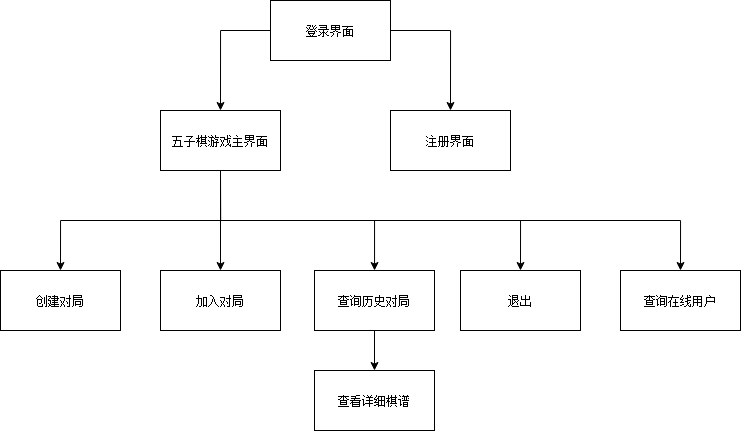
\includegraphics[width=\textwidth]{pictures/1}
    \caption{客户端总体功能}
\end{figure}
服务端程序设计达成的功能说明:
\begin{enumerate}
    \item 提供用户登录、注册服务
    \item 提供用户创建对局服务
    \item 提供用户加入对局服务
    \item 提供用户查询历史对局服务
    \item 提供用户查询对局棋谱服务
    \item 提供用户查询在线用户服务
    \item 提供对局的过程支持(包含放置棋子、回合转换和输赢判定)
\end{enumerate}
\begin{figure}[htbp]
    \centering
    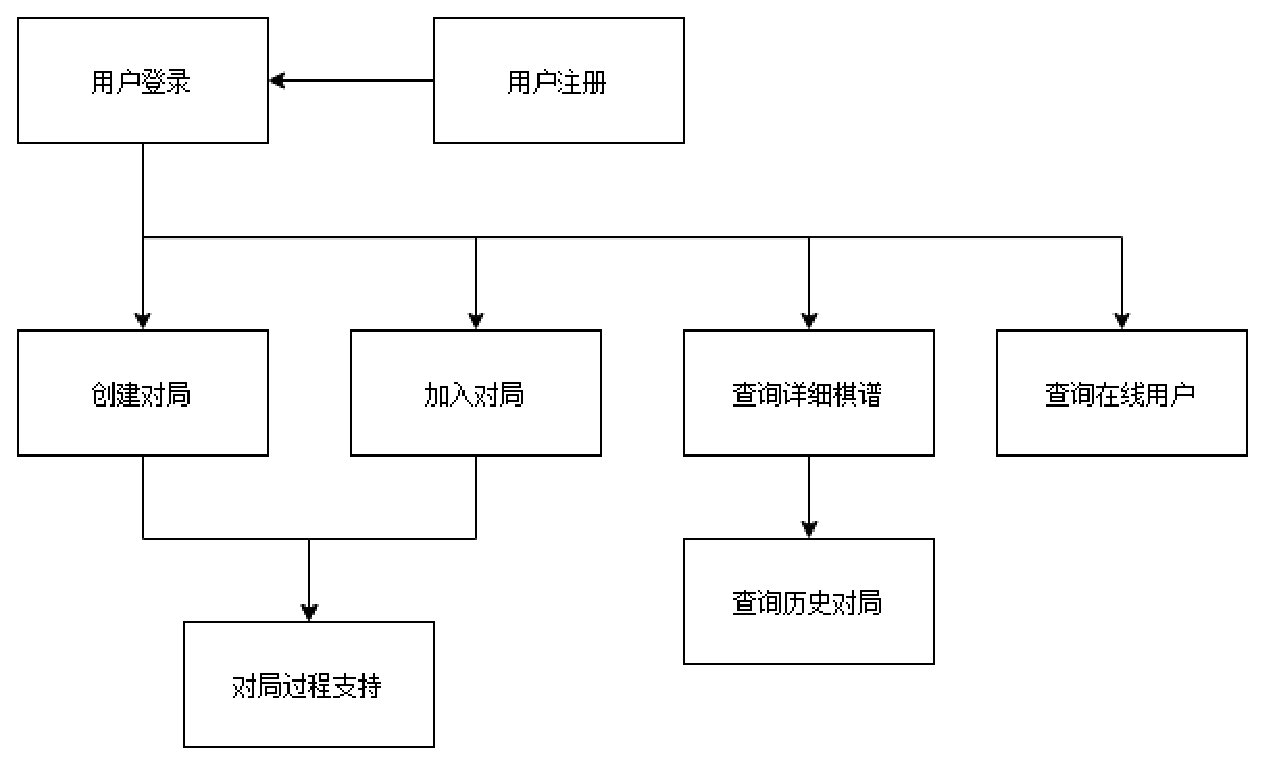
\includegraphics[width=\textwidth]{pictures/2}
    \caption{服务端总体功能}
\end{figure}
\subsection{流程图设计}
\newpage
\begin{figure}[H]
    \centering
    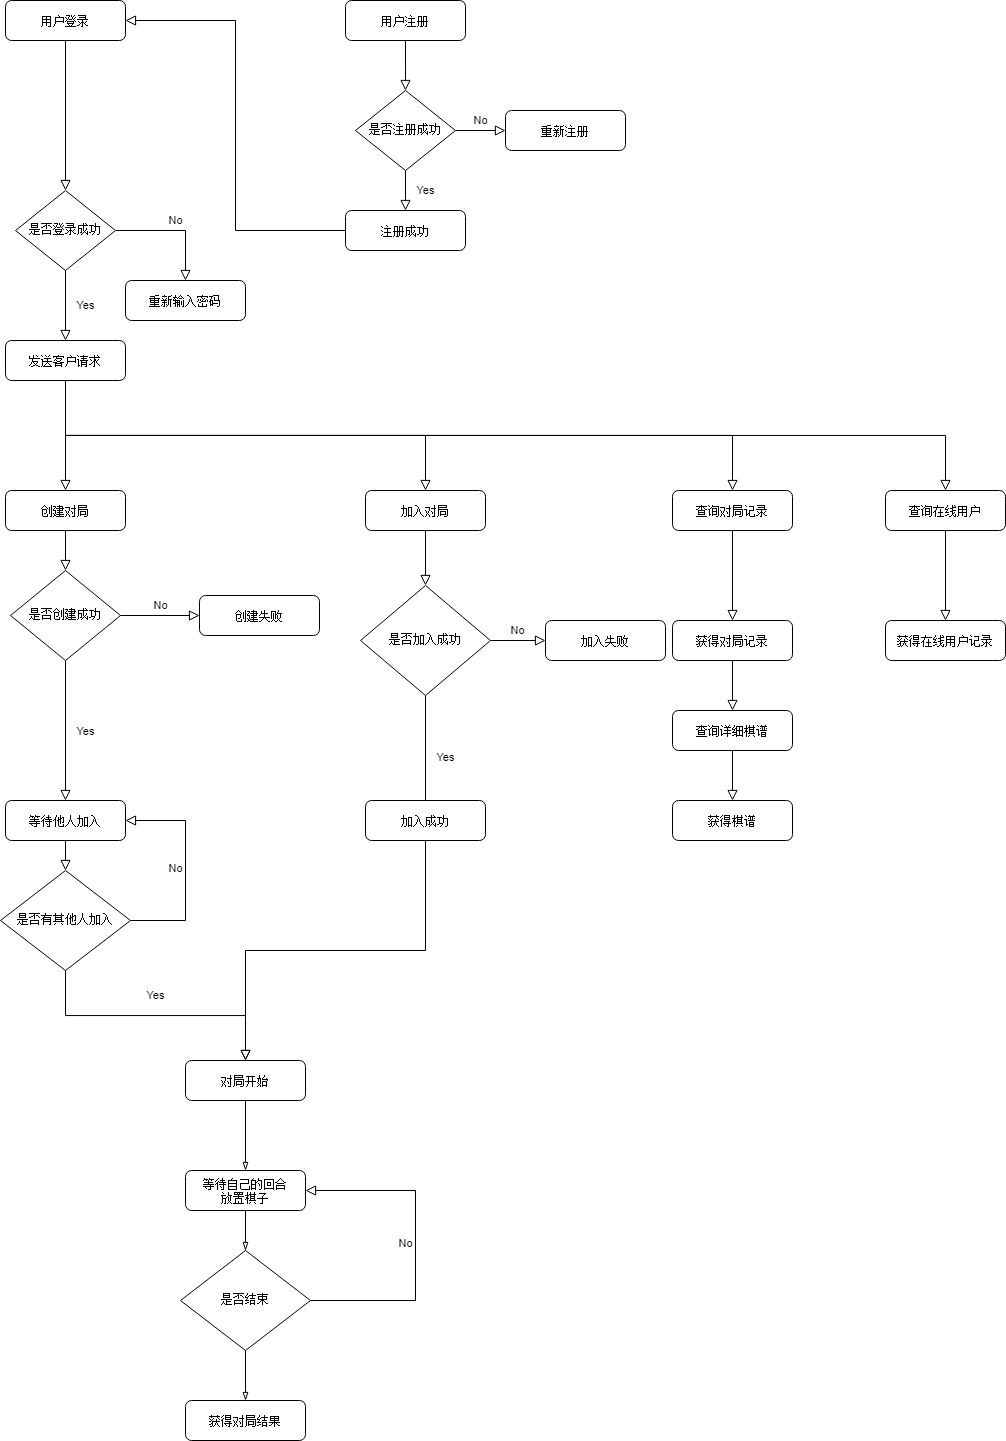
\includegraphics[width=\textwidth]{pictures/4}
    \caption{客户端流程设计}
\end{figure}
\newpage
\begin{figure}[H]
    \centering
    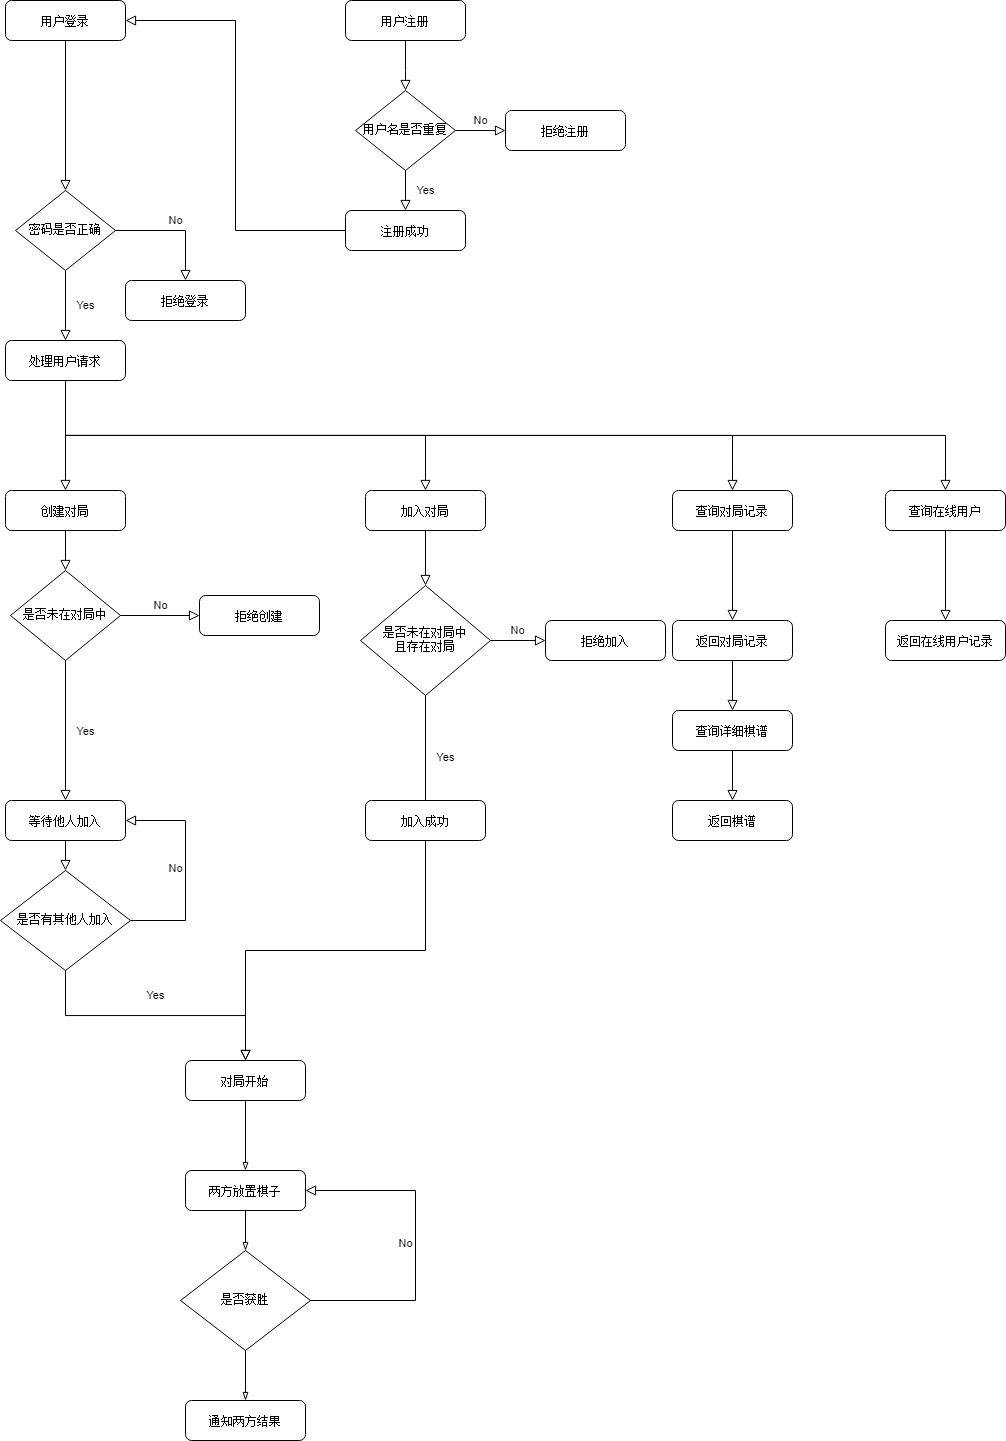
\includegraphics[width=\textwidth]{pictures/3}
    \caption{服务端流程设计}
\end{figure}
\section{详细设计}
\subsection{客户端设计}
\subsubsection{登录界面与功能的设计}
登录界面主要采用了用户名输入框、密码输入框、登录按钮和注册按钮这4个控件。
当点击登录按钮时,LoginHandler会读取输入的用户名和密码,然后上传给服务端。
在上传之前,还会检查是否已经登录,若已经登陆,就会弹出提示框提醒用户。
如果服务端回应密码输入错误,也会弹出提示框提醒用户
登录成功后,跳转到主界面。
用户还可以通过注册按钮调转到注册界面进行注册。\\
登录控件代码框架如下:
\begin{listing}[htb]
    \caption{登录界面控件}
    \begin{minted}{Java}
    public class LoginHandler {
        //用户名输入框
        @FXML
        private TextField usernameField; 
        //密码输入框
        @FXML 
        private PasswordField passwordField;
        //登录按钮绑定方法
        private void handleLogin() {}
        //注册按钮绑定方法
        private void handleRegister() {}
        //弹出提示框方法
        private void showAlert(Alert.AlertType alertType, 
        String title, String message) {}
    }
    \end{minted}
\end{listing}
\newpage
\begin{figure}[H]
    \centering
    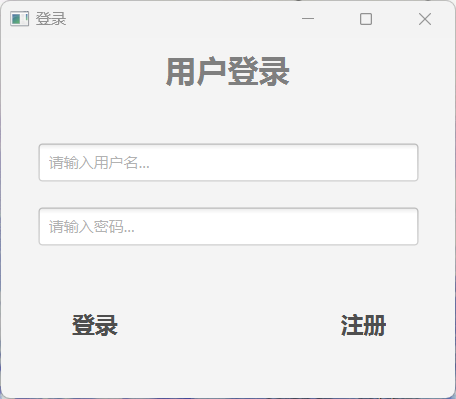
\includegraphics[width=\textwidth]{pictures/5}
    \caption{登录界面}
\end{figure}
\subsubsection{注册界面与功能的设计}
注册界面录主要采用了用户名输入框、密码输入框注册和按钮这3个控件。
当点击注册按钮时,RegisterHandler会读取输入的用户名和密码,然后上传给服务端。
如果服务器回应用户名重复,会弹出提示框提醒用户重新输入用户名,如果登录成功,会跳转回登录页面\\
注册控件代码框架如下:
\begin{listing}[htb]
    \caption{注册界面控件}
    \begin{minted}{Java}
    public class RegisterHandler {
        @FXML 
        private TextField usernameField;
        @FXML 
        private PasswordField passwordField;
        //绑定注册按钮方法
        @FXML
        private void handleRegister() {}
        //弹出提示框方法
        private void showAlert(Alert.AlertType alertType, 
        String title, String message) {}
    }
    \end{minted}
\end{listing}
\begin{figure}[H]
    \centering
    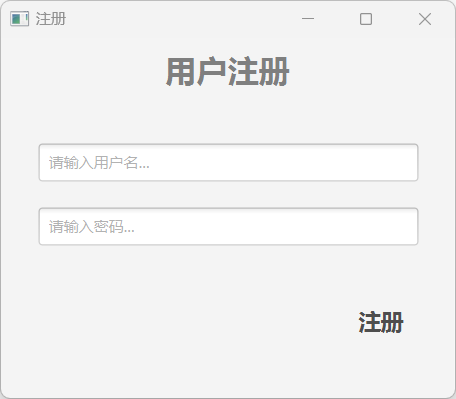
\includegraphics[width=0.8\textwidth]{pictures/6}
    \caption{注册界面}
\end{figure}
\subsubsection{主界面与功能的设计}
主界面主要采用了5个按钮控件来提供不同的功能。
\begin{figure}[H]
    \centering
    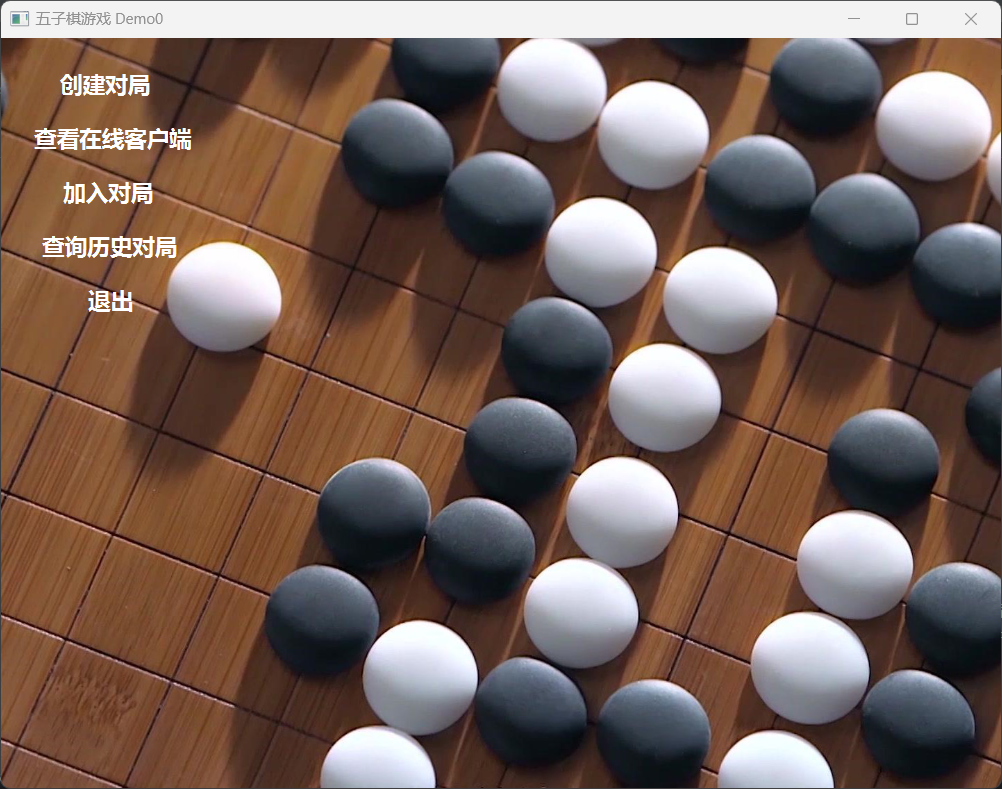
\includegraphics[width=0.8\textwidth]{pictures/7}
    \caption{主界面}
\end{figure}
\paragraph{创建对局按钮}
当点击了创建对局按钮时,客户端向服务端发送创建对局请求,获取服务端许可后,创建对局页面。
关于对局页面,将在五子棋棋盘界面与功能的设计中介绍。
\paragraph{查看在线客户端}
当点击了查看在线客户端页面后,客户端向服务端发送查看在线客户端请求,获取服务端结果并展示。
\begin{figure}[H]
    \centering
    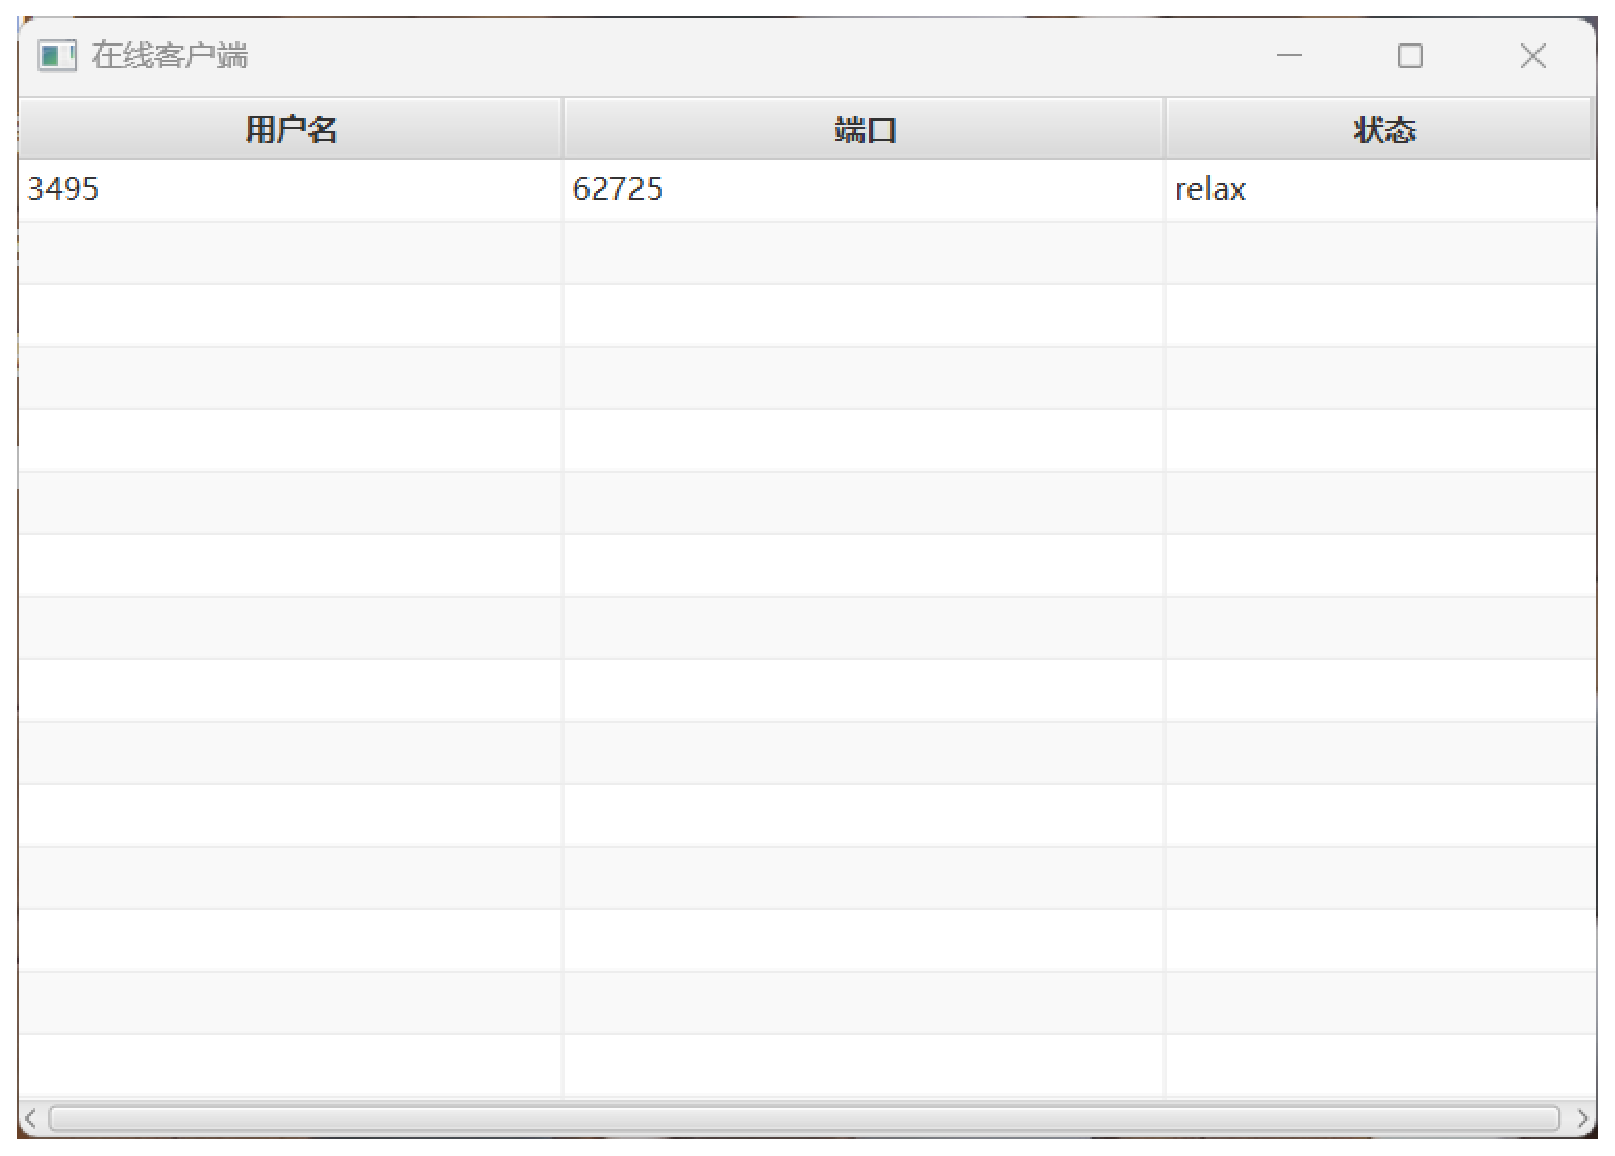
\includegraphics[width=0.8\textwidth]{pictures/8}
    \caption{在线客户端展示表}
\end{figure}
\paragraph{加入对局}
当点击了加入对局按钮,客户端向服务端发送加入对局请求,获取服务端加入许可后,创建对局页面,
若服务端通知当前没有可加入的对局,客户端弹出相关提示提醒用户。
\paragraph{查询历史对局按钮}
当点击了查询历史对局按钮,客户端向服务端发送查看历史对局请求,获取服务端结果并展示。
\begin{figure}[H]
    \centering
    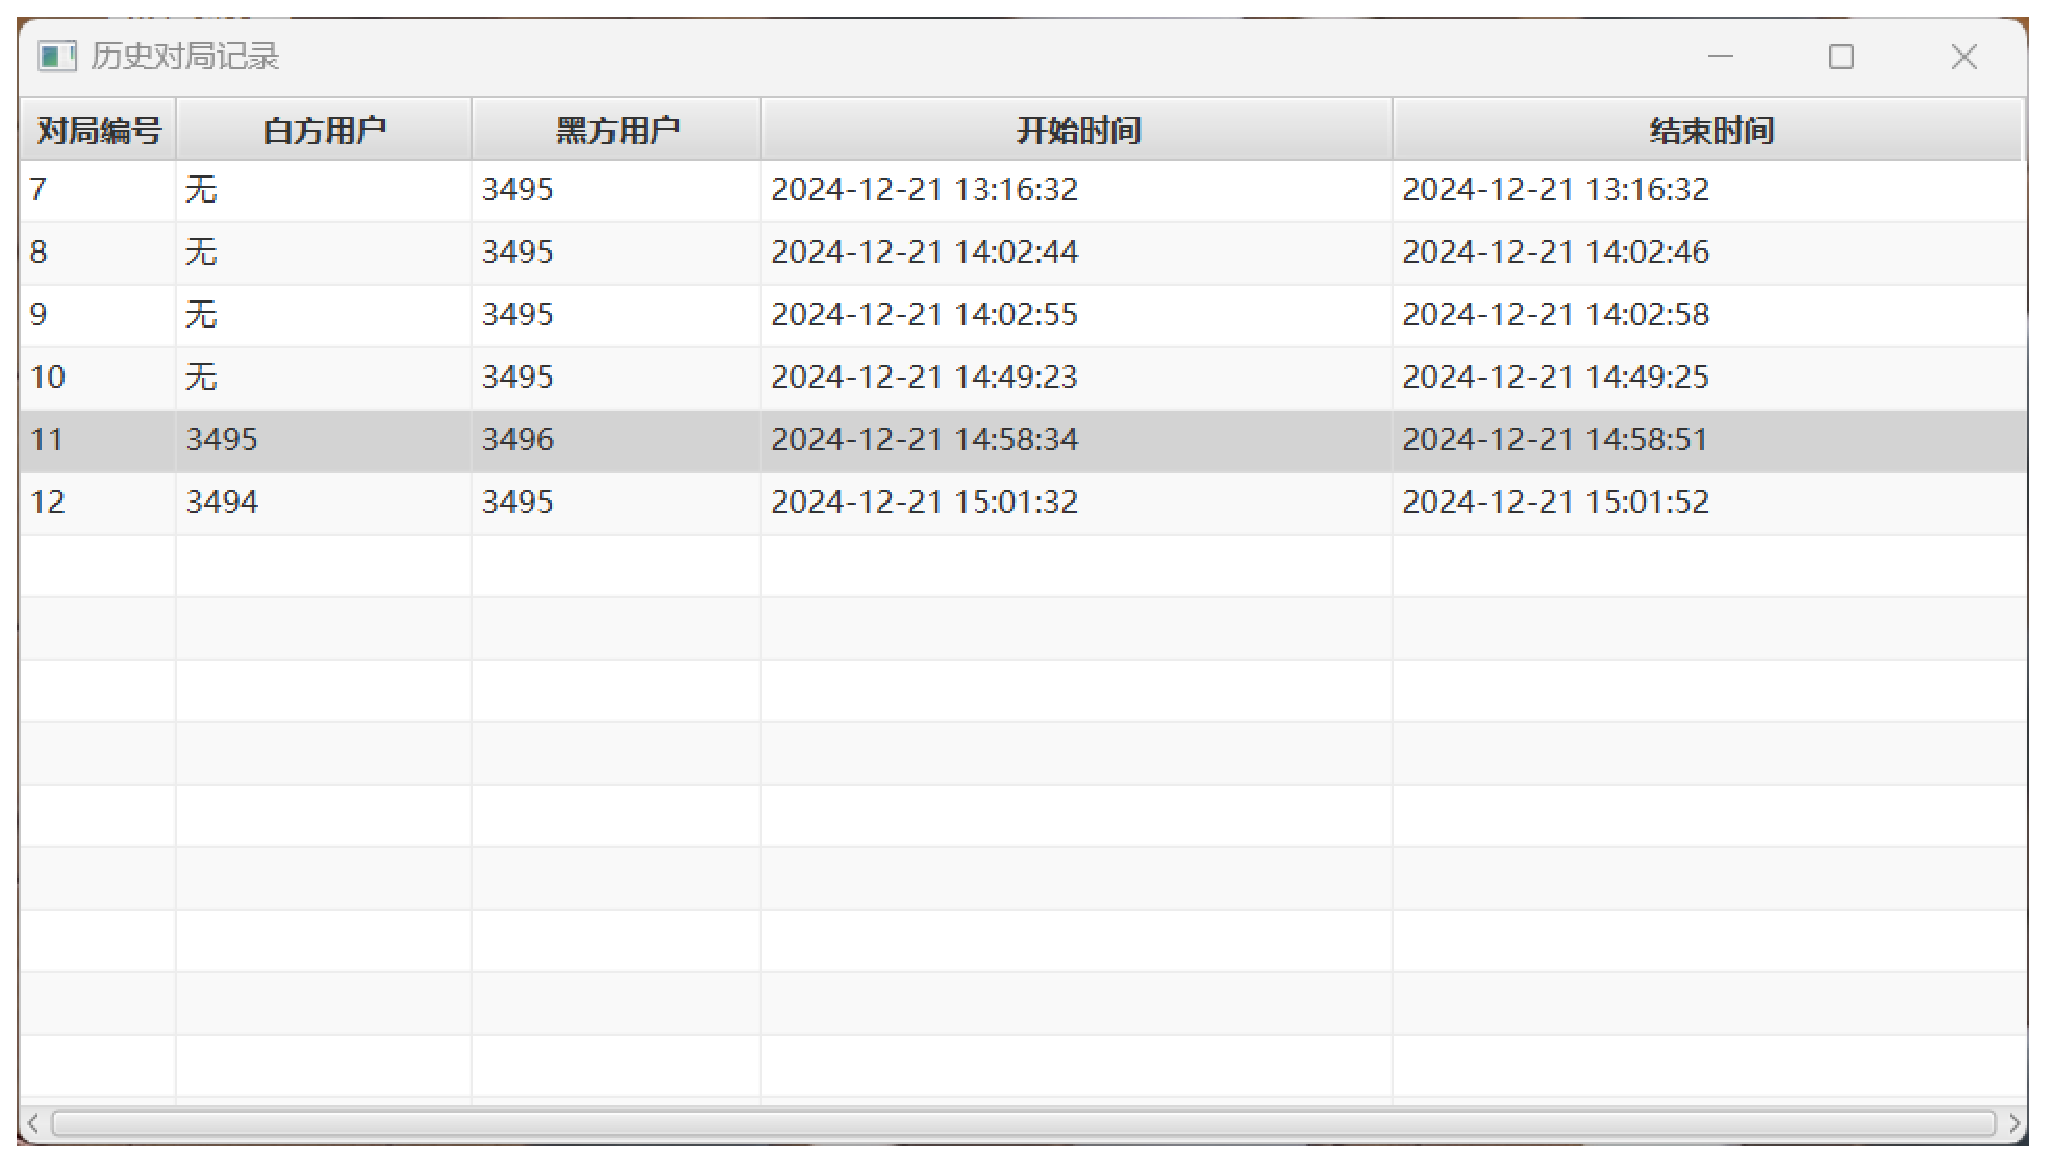
\includegraphics[width=0.8\textwidth]{pictures/9}
    \caption{历史对局展示表}
\end{figure}
在此基础上,用户双击对应的行,客户端将向服务端发送查询具体棋谱请求,获取服务端结果并展示
\begin{figure}[H]
    \centering
    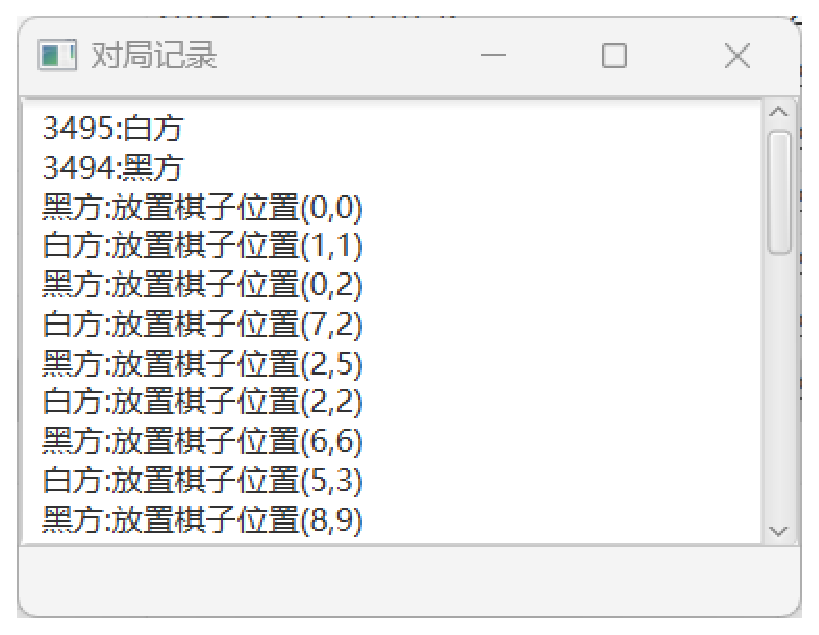
\includegraphics[width=0.6\textwidth]{pictures/10}
    \caption{棋谱展示}
\end{figure}
\paragraph{退出按钮}
当用户点击退出按钮时,客户端程序断开与服务端点连接,并结束程序。
\newpage
主界面控件的代码框架如下:
\begin{listing}[H]
    \caption{注册界面控件}
    \begin{minted}{Java}
        public class MainHandler {
            // 客户端与服务端通信的Socket
            Socket socket;
            // 客户端通过out向服务端发送信息
            PrintWriter out;
            // 绑定查询在线用户按钮方法
            // 其他辅助成员变量略去
            @FXML
            protected void queryClientList(ActionEvent event) {}
            // 绑定查询用户历史对局按钮方法
            @FXML
            protected void queryAllHistory() {}
            // 绑定用户退出按钮方法
            @FXML
            public void quit(ActionEvent event) {}
            // 绑定用户创建对局按钮方法
            @FXML
            protected void createGame(ActionEvent event) {}
            // 绑定用户加入对局按钮方法
            @FXML
            protected void joinGame(ActionEvent event) {}
            //其他辅助成员函数略去
        }
    \end{minted}
\end{listing}
\subsubsection{五子棋棋盘界面与功能的设计}
五子棋棋盘类继承了JavaFx的Pane控件类,绑定了鼠标点击事件。
点击了创建对局之后,若有人加入;或是加入了别人创建的对局,服务端就会向客户端发送对局开始的回应,随后客户端创建
五子棋棋盘界面,并且用弹窗提示用户持黑子或是白子。
考虑到用户会多次创建对局,因而在主界面的控件类中包含了一个五子棋棋盘类的成员对象,方便在对局终止之后对其进行重置。
\begin{figure}[H]
    \centering
    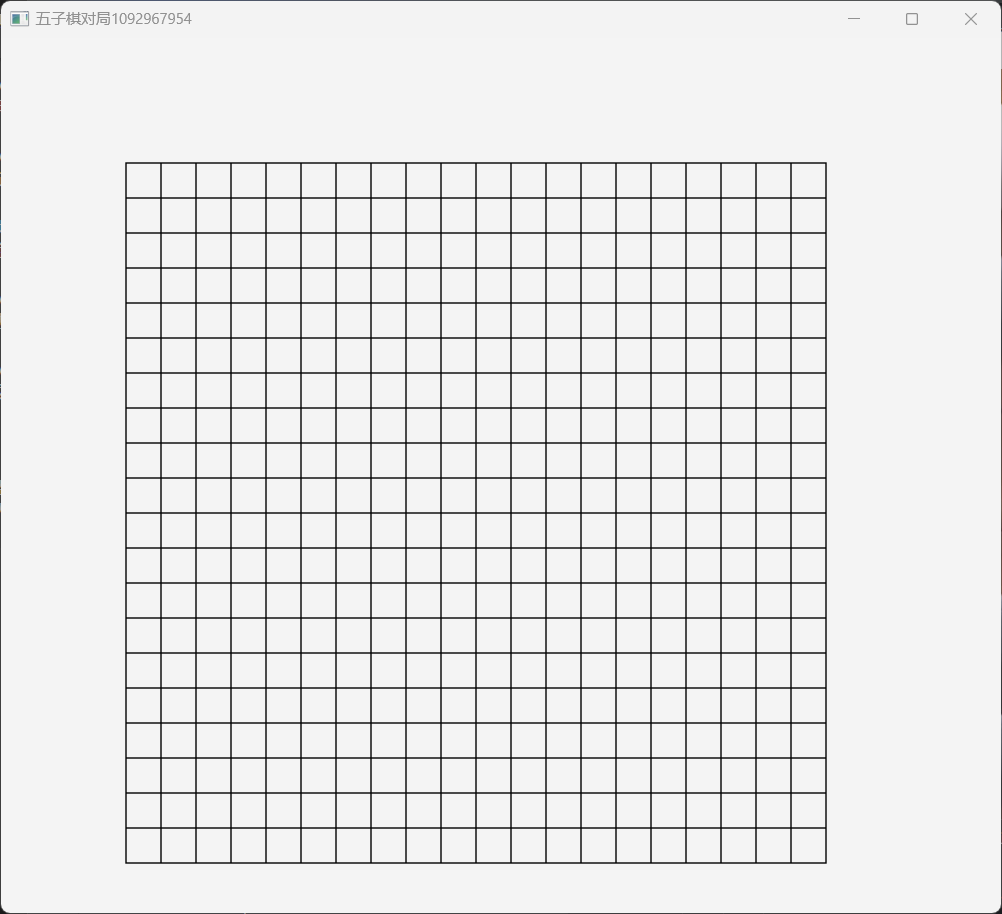
\includegraphics[width=0.6\textwidth]{pictures/11}
    \caption{五子棋棋盘界面}
\end{figure}
开始对局之后,用户在棋盘上点击,客户端会获取用户点击的棋盘坐标,发送给服务端,服务端验证坐标的合法性后
记录下坐标,判断是否对局结束,之后再通知客户端绘制对应坐标点的棋子。对局结束后,客户端收到服务端的结果
通过弹窗提示用户,然后关闭棋盘。如果一方在对局中途退出,服务端会通知另一方的客户端退出对局,
之后两方棋盘窗口均关闭
\subsubsection{客户端接收信息线程的设计}
考虑到发送与接收的异步性,客户端还需要独立运行一个接收线程来专门负责接收服务器发来的信息。
这个线程不涉及图形窗口,它的代码框架如下:
\begin{listing}[H]
    \caption{注册界面控件}
    \begin{minted}{Java}
    public class ReceiveMessageHandler implements Runnable {
        // 与服务端通信的socket
        Socket socket;
        // 负责接收服务器信息
        BufferedReader in;
        // 和主界面线程共享的窗口
        Stage stage;
        // 创建该线程的主线程
        MainHandler mainHandler;
        // 其他负责成员对象略去
        // 接收服务端响应创建对局页面
        public void createGame(String response) {}
        // 接收服务端响应绘制棋子
        public void placeChess(String response) {}
        // 接收服务端响应退出对局
        public void quitGame() {}
        // 接收服务端响应终止对局
        public void overGame() {}
        // 接收服务端响应获取并展示在线客户端
        public void clientList(String response) {}
        // 接收服务器响应设置登录状态
        public void login() {}
        // 接收服务器响应开始对局
        public void startGame(String response) {}
        // 接收服务器响应获取并展示该用户所以对局记录
        public void showAllHistory(String response) {}
        // 接收服务器响应获取并展示具体棋谱
        public void showRecord(String response) {}
        // 其他辅助成员函数略去
    }
    \end{minted}
\end{listing}
\subsection{服务端设计}
\subsubsection{与客户端交互模块的设计}
服务端的根本逻辑是接收客户端请求并响应。为了满足不同客户端的并发请求,服务端采用一个客户端对应一个服务端线程\ (ClientHandler)的方式
来处理。这样的设计使得服务端能够同时处理多个用户多个对局。考虑并发场景的临界资源访问问题,在一些共享的成员变量\ (如
当前在线用户表、当前可加入对局表和正在进行对局表)操作时
服务端使用synchronized关键字来保证数据一致性。
以下是ClientHandler的代码框架:
\begin{listing}[H]
    \caption{注册界面控件}
    \begin{minted}{Java}
    public class ClientHandler implements Runnable {
        // 登录用户信息,包含用户名、id、端口等
        private final ClientInfo clientInfo;
        // 在线用户表
        private final Map<String, ClientInfo> clients;
        // 等待开始的对局表
        private final Map<Integer, Game> waitingGames;
        // 正在进行的对局表
        private final Map<Integer, Game> runningGames;
        // 在线用户的用户名表(用于快速查询用户是否登录)
        private final Set<String> loggedUsers;
        // 发送在线客户端表到客户端
        public void sendClientsList(PrintWriter out) {}
        // 发生对局记录到客户端
        public void queryAllHistory(PrintWriter out) {}
        // 通知客户端是否可以创建对局
        public void createGame(PrintWriter out) {}
        // 通知客户端是否可以加入对局
        public void joinGame(PrintWriter out) {}
        // 通知客户端是否可以在特定位置放置棋子
        public void placeChess(PrintWriter out, String message) {}
        // 通知客户端退出对局(对局中止)
        public void quitGame(PrintWriter out) {}
        // 通知客户端结束对局(对局结束)
        public void overGame() {}
        // 通知客户端是否登录成功
        public void login(PrintWriter out, String inputLine) {}
        // 通知客户端是否注册成功
        public void register(PrintWriter out, String inputLine) {}
        // 发生对局棋谱到客户端
        public void queryRecord(PrintWriter out, String inputLine) {}
    }
    \end{minted}
\end{listing}
除此之外,考虑到用户信息和对局数据的持久性,服务端还采用MySQL数据库来储存对局数据和用户信息,使得用户登录功能、用户
查询历史对局功能和用户查询对局棋谱功能得以实现。服务端设计了DataBaseManager类来与数据库进行交互。
以下是DataBaseManager的代码框架:
\begin{listing}[H]
    \caption{注册界面控件}
    \begin{minted}{Java}
    public class DatabaseManager {
        private static final String DB_URL = "略去";
        private static final String DB_USER = "略去";
        private static final String DB_PASSWORD = "略去";
        // 通过con对数据库进行操作
        private static Connection con;
        // 查询是否存在该用户,如果有就返回其id,否则返回-1
        public static Integer login(String username, String password) {}
        // 往数据库插入该用户的信息,如果成功返回true
        public static Boolean register(String username, String password) {}
        // 往数据库中插入对局的记录
        public static void gameRecord(String black_username, String white_username,
            String content, Timestamp start_time, Timestamp end_time) {}
        // 查询某个用户参与的对局记录并返回记录(不包含棋谱)的列表
        public static List<Record> queryAllRecords(String user_name) {}
        // 查询某个id的记录并返回记录的棋谱
        public static String queryRecord(int id) {}
    }
    \end{minted}
\end{listing}
\subsubsection{数据库的设计}
\paragraph{用户表设计}用户表由自增的id、表示用户名的字符串username和表示密码的字符串password构成,以下是建表语句:
\begin{listing}[H]
    \begin{minted}{sql}
    CREATE TABLE `user` (
        `username` varchar(50) NOT NULL,
        `password` varchar(45) CHARACTER SET latin1 NOT NULL,
        `id` int(11) NOT NULL AUTO_INCREMENT,
        PRIMARY KEY (`id`,`username`),
        UNIQUE KEY `username_UNIQUE` (`username`)
    ) ENGINE=InnoDB AUTO_INCREMENT=13 DEFAULT CHARSET=utf8mb4
    \end{minted}
    \caption{用户表设计}
\end{listing}
\paragraph{对局记录表设计}对局记录表由自增的id、表示黑方用户名的字符串black\_ username、表示白方用户名的字符串white\_username、
表示棋谱内容的字符串content、表示开始时间的start\_time和表示结束时间的end\_time组成,以下是建表语句:

\begin{listing}[H]
    \begin{minted}{sql}
    CREATE TABLE `record` (
        `id` int(11) NOT NULL AUTO_INCREMENT,
        `black_username` varchar(50) DEFAULT NULL,
        `white_username` varchar(50) DEFAULT NULL,
        `content` text NOT NULL,
        `start_time` datetime NOT NULL,
        `end_time` datetime NOT NULL,
        PRIMARY KEY (`id`)
        ) ENGINE=InnoDB AUTO_INCREMENT=19 DEFAULT CHARSET=utf8mb4
    \end{minted}
    \caption{用户表设计}
\end{listing}
\section{测试与运行}
\subsection{程序测试}
% Please add the following required packages to your document preamble:
% \usepackage{multirow}
% \usepackage{longtable}
% Note: It may be necessary to compile the document several times to get a multi-page table to line up properly
{
    \scriptsize

\begin{longtable}{|c|c|c|c|}
    \hline
    测试场景 &
      测试步骤 &
      测试样例 &
      测试结果 \\ \hline
    \endfirsthead
    %
    \endhead
    %
    \multirow{2}{*}{用户登录} &
      \begin{tabular}[c]{@{}c@{}}1.打开客户端\\ 2.输入正确用户名和密码\\ 3.点击登录\end{tabular} &
      \begin{tabular}[c]{@{}c@{}}用户名:3495\\ 密码:123456\end{tabular} &
      \begin{tabular}[c]{@{}c@{}}通过:\\ 客户端跳转到主界面\end{tabular} \\ \cline{2-4} 
     &
      \begin{tabular}[c]{@{}c@{}}1.打开客户端\\ 2.输入错误用户名和密码\\ 3.点击登录\end{tabular} &
      \begin{tabular}[c]{@{}c@{}}用户名:3333\\ 密码:123456\end{tabular} &
      \begin{tabular}[c]{@{}c@{}}通过:\\ 客户端弹窗显示密码错误\end{tabular} \\ \hline
    \multirow{4}{*}{用户注册} &
      \begin{tabular}[c]{@{}c@{}}1.打开客户端\\ 2.输入服务端没有的用户名\\ 3.输入密码\\ 4.点击注册\end{tabular} &
      \begin{tabular}[c]{@{}c@{}}用户名:3496\\ 密码:123456\end{tabular} &
      \begin{tabular}[c]{@{}c@{}}通过:\\ 客户端弹窗显示注册成功,\\ 之后跳转到登录页面\end{tabular} \\ \cline{2-4} 
     &
      \begin{tabular}[c]{@{}c@{}}1.打开客户端\\ 2.输入服务端存在的用户名\\ 3.输入密码\\ 4.点击注册\end{tabular} &
      \begin{tabular}[c]{@{}c@{}}用户名:3495\\ 密码:123456789\end{tabular} &
      \begin{tabular}[c]{@{}c@{}}通过:\\ 客户端弹窗显示用户名重复\end{tabular} \\ \cline{2-4} 
     &
      \begin{tabular}[c]{@{}c@{}}1.注册成功\\ 2.尝试用注册时的账号密码登录\end{tabular} &
      \begin{tabular}[c]{@{}c@{}}用户名:3496\\ 密码:123456\end{tabular} &
      \begin{tabular}[c]{@{}c@{}}通过:\\ 客户端跳转到主界面\end{tabular} \\ \cline{2-4} 
     &
      \begin{tabular}[c]{@{}c@{}}1.注册失败\\ 2.尝试用注册时的账号密码登陆\end{tabular} &
      \begin{tabular}[c]{@{}c@{}}用户名:3495\\ 密码:123456789\end{tabular} &
      \begin{tabular}[c]{@{}c@{}}通过:\\ 客户端弹窗显示密码错误\end{tabular} \\ \hline
    \multirow{4}{*}{用户创建对局} &
      \begin{tabular}[c]{@{}c@{}}1.登录后进入主界面\\ 2.点击创建对局按钮\end{tabular} &
      \begin{tabular}[c]{@{}c@{}}用户名:3495\\ 密码:123456\end{tabular} &
      \begin{tabular}[c]{@{}c@{}}通过:\\ 客户端弹出对局界面\end{tabular} \\ \cline{2-4} 
     &
      \begin{tabular}[c]{@{}c@{}}1.登录后进入主界面\\ 2.点击创建对局按钮\\ 3.再次点击创建对局按钮\end{tabular} &
      \begin{tabular}[c]{@{}c@{}}用户名:3495\\ 密码:123456\end{tabular} &
      \begin{tabular}[c]{@{}c@{}}通过:\\ 客户端第一次弹出对局界面\\ 第二次弹窗提示已经在对局中\end{tabular} \\ \cline{2-4} 
     &
      \begin{tabular}[c]{@{}c@{}}1.客户端A登录后进入主界面\\ 2.点击创建对局按钮\\ 3.客户端B登录后进入主界面\\ 4.点击加入对局按钮\\ 客户端A再次点击创建对局按钮\end{tabular} &
      \begin{tabular}[c]{@{}c@{}}A\\ 用户名:3495\\ 密码:123456\\ B\\ 用户名:3495\\ 密码:123456\end{tabular} &
      \begin{tabular}[c]{@{}c@{}}通过:\\ A客户端第一次弹出对局界面\\ 第二次提示对局开始\\ 第三次弹窗提示已经在对局中\\ B客户端弹出对局界面和对局开始提示\end{tabular} \\ \cline{2-4} 
     &
      \begin{tabular}[c]{@{}c@{}}1.客户端A登录后进入主界面\\ 2.点击创建对局按钮\\ 3.客户端B登录后进入主界面\\ 4.点击加入对局按钮\\ 客户端B点击创建对局按钮\end{tabular} &
      \begin{tabular}[c]{@{}c@{}}A\\ 用户名:3495\\ 密码:123456\\ B\\ 用户名:3495\\ 密码:123456\end{tabular} &
      \begin{tabular}[c]{@{}c@{}}通过:\\ A客户端第一次弹出对局界面\\ 第二次提示对局开始\\ B客户端第一次弹出对局界面和对局开始提示\\ 第二次弹窗提示已经在对局中\end{tabular} \\ \hline
    \multirow{2}{*}{用户加入} &
      \begin{tabular}[c]{@{}c@{}}1.登录后进入主界面\\ 2.点击创建对局按钮\end{tabular} &
      \begin{tabular}[c]{@{}c@{}}用户名:3495\\ 密码:123456\end{tabular} &
      \begin{tabular}[c]{@{}c@{}}通过:\\ 客户端弹窗提示没有可加入的对局\end{tabular} \\ \cline{2-4} 
     &
      \begin{tabular}[c]{@{}c@{}}1.客户端A登录后进入主界面\\ 2.点击创建对局按钮\\ 3.客户端B登录后进入主界面\\ 4.点击加入对局按钮\end{tabular} &
      \begin{tabular}[c]{@{}c@{}}A\\ 用户名:3495\\ 密码:123456\\ B\\ 用户名:3495\\ 密码:123456\end{tabular} &
      \begin{tabular}[c]{@{}c@{}}通过:\\ A客户端第一次弹出对局界面\\ 第二次提示对局开始\\ B客户端弹出对局界面和对局开始提示\end{tabular} \\ \hline
    \multirow{5}{*}{\begin{tabular}[c]{@{}c@{}}用户端进行对局\\ 服务端进行记录\end{tabular}} &
      \begin{tabular}[c]{@{}c@{}}1.客户端A创建对局\\ 2.客户端B加入对局\\ 3.A、B轮流下棋直到一方获胜\end{tabular} &
      \begin{tabular}[c]{@{}c@{}}A\\ 用户名:3495\\ 密码:123456\\ B\\ 用户名:3495\\ 密码:123456\end{tabular} &
      \begin{tabular}[c]{@{}c@{}}通过\\ 两方客户端弹窗提示结果\\ 关闭弹窗后\\ 对局界面关闭\\ 服务端数据库记录的棋谱包含\\ A、B下棋过程以及结果\end{tabular} \\ \cline{2-4} 
     &
      \begin{tabular}[c]{@{}c@{}}1.客户端A创建对局\\ 2.客户端B加入对局\\ 3.轮到A的回合\\ 4.A点击已经下过的位置\\ 5.A点击没下过的位置\end{tabular} &
      \begin{tabular}[c]{@{}c@{}}A\\ 用户名:3495\\ 密码:123456\\ B\\ 用户名:3495\\ 密码:123456\end{tabular} &
      \begin{tabular}[c]{@{}c@{}}通过\\ 客户端A第一次点击后没有反应\\ 第二次点击后出现棋子\\ 服务端未收到A的第一次点击记录\end{tabular} \\ \cline{2-4} 
     &
      \begin{tabular}[c]{@{}c@{}}1.客户端A创建对局\\ 2.客户端B加入对局\\ 3.轮到B的回合\\ 4.A点击没下过的位置\end{tabular} &
      \begin{tabular}[c]{@{}c@{}}A\\ 用户名:3495\\ 密码:123456\\ B\\ 用户名:3495\\ 密码:123456\end{tabular} &
      \begin{tabular}[c]{@{}c@{}}通过\\ 客户端A弹窗提示当前尚未轮到\\ 服务端未收到A的点击记录\end{tabular} \\ \cline{2-4} 
     &
      \begin{tabular}[c]{@{}c@{}}1.客户端A创建对局\\ 2.客户端B加入对局\\ 3.A、B轮流下棋\\ 4.在没结束时A退出\end{tabular} &
      \begin{tabular}[c]{@{}c@{}}A\\ 用户名:3495\\ 密码:123456\\ B\\ 用户名:3495\\ 密码:123456\end{tabular} &
      \begin{tabular}[c]{@{}c@{}}通过\\ 客户端A和客户端B同时退出对局界面\\ 服务端数据库中记录的棋谱包含\\ A、B的下棋过程以及最后对局中止\end{tabular} \\ \cline{2-4} 
     &
      \begin{tabular}[c]{@{}c@{}}1.客户端A创建对局\\ 2.客户端A关闭对局界面\end{tabular} &
      \begin{tabular}[c]{@{}c@{}}A\\ 用户名:3495\\ 密码:123456\end{tabular} &
      \begin{tabular}[c]{@{}c@{}}通过\\ 客户端A退出对局界面\\ 服务端数据库中记录的棋谱只包含\\ A的用户名以及对局中止\end{tabular} \\ \hline
    \multirow{2}{*}{用户查询在线客户端} &
      \begin{tabular}[c]{@{}c@{}}1.客户端A登录\\ 2.A查询在线客户端\\ 3.客户端B登录\\ 4.A、B查询在线客户端\end{tabular} &
      \begin{tabular}[c]{@{}c@{}}A\\ 用户名:3495\\ 密码:123456\\ B\\ 用户名:3495\\ 密码:123456\end{tabular} &
      \begin{tabular}[c]{@{}c@{}}通过\\ 客户端A第一次显示只有A的登录记录\\ 客户端A第二次显示A、B登录记录\\ 客户端B显示A、B的登录记录\end{tabular} \\ \cline{2-4} 
     &
      \begin{tabular}[c]{@{}c@{}}1.客户端A登录\\ 2.客户端B登录\\ 3.A查询在线客户端\\ 4.B退出\\ 5.A查询在线客户端\end{tabular} &
      \begin{tabular}[c]{@{}c@{}}A\\ 用户名:3495\\ 密码:123456\\ B\\ 用户名:3495\\ 密码:123456\end{tabular} &
      \begin{tabular}[c]{@{}c@{}}通过\\ 客户端A第一次显示A、B的登录记录\\ 客户端A第二次显示A登录记录\end{tabular} \\ \hline
    \multirow{3}{*}{用户查询历史对局记录} &
      \begin{tabular}[c]{@{}c@{}}1.客户端A登录\\ 2.客户端A查询历史对局记录\\ 3.客户端B登录\\ 4.客户端A、B进行对局至结束\\ 5.客户端A查询历史对局记录\end{tabular} &
      \begin{tabular}[c]{@{}c@{}}A\\ 用户名:3495\\ 密码:123456\\ B\\ 用户名:3495\\ 密码:123456\end{tabular} &
      \begin{tabular}[c]{@{}c@{}}通过\\ 客户端A第一次查询到之前的历史对局记录\\ 客户端A第二次查询到历史对局记录包含刚发生的对局\end{tabular} \\ \cline{2-4} 
     &
      \begin{tabular}[c]{@{}c@{}}1.客户端A登录\\ 2.客户端A查询历史对局记录\\ 4.客户端A创建对局后退出\\ 5.客户端A查询历史对局记录\end{tabular} &
      \begin{tabular}[c]{@{}c@{}}A\\ 用户名:3495\\ 密码:123456\end{tabular} &
      \begin{tabular}[c]{@{}c@{}}通过\\ 客户端A第一次查询到之前的历史对局记录\\ 客户端A第二次查询到历史对局记录包含刚创建的对局\end{tabular} \\ \cline{2-4} 
     &
      \begin{tabular}[c]{@{}c@{}}1.客户端A登录\\ 2.客户端A查询历史对局记录\\ 3.客户端B登录\\ 4.客户端A、B进行对局,中途退出\\ 5.客户端A查询历史对局记录\end{tabular} &
      \begin{tabular}[c]{@{}c@{}}A\\ 用户名:3495\\ 密码:123456\\ B\\ 用户名:3495\\ 密码:123456\end{tabular} &
      \begin{tabular}[c]{@{}c@{}}通过\\ 客户端A第一次查询到之前的历史对局记录\\ 客户端A第二次查询到历史对局记录包含刚退出的对局\end{tabular} \\ \hline
    \multirow{2}{*}{用户查询记录棋谱} &
      \begin{tabular}[c]{@{}c@{}}1.客户端A登录\\ 2.客户端A查询历史对局记录\\ 3.客户端A双击一条记录\end{tabular} &
      \begin{tabular}[c]{@{}c@{}}A\\ 用户名:3495\\ 密码:123456\end{tabular} &
      \begin{tabular}[c]{@{}c@{}}通过\\ 客户端A弹窗显示该记录的棋谱\end{tabular} \\ \cline{2-4} 
     &
      \begin{tabular}[c]{@{}c@{}}1.客户端A登录\\ 2.客户端A查询历史对局记录\\ 3.客户端A记录外的其他区域\end{tabular} &
      \begin{tabular}[c]{@{}c@{}}A\\ 用户名:3495\\ 密码:123456\end{tabular} &
      \begin{tabular}[c]{@{}c@{}}通过\\ 客户端A双击没有反应\end{tabular} \\ \hline
    
    \caption{程序测试表}
    \end{longtable}
}
\subsection{程序运行}
运行程序,进入用户登录页面
\begin{figure}[H]
    \centering
    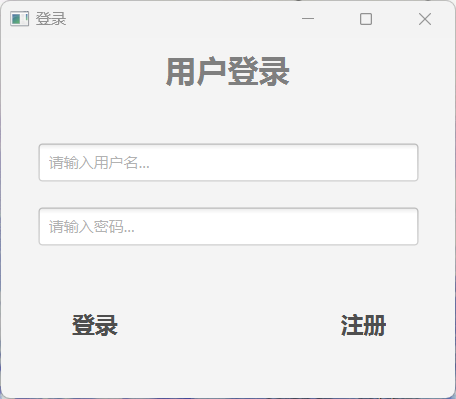
\includegraphics[width=0.5\textwidth]{pictures/5}
    \caption{登录界面}
\end{figure}
点击注册,进入用户注册页面
\begin{figure}[H]
    \centering
    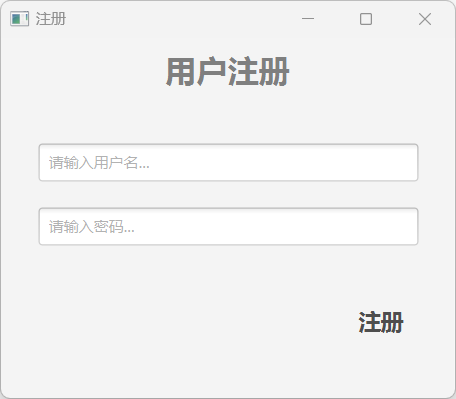
\includegraphics[width=0.5\textwidth]{pictures/6}
    \caption{注册界面}
\end{figure}
输入用户名和密码,完成注册
\begin{figure}[H]
    \centering
    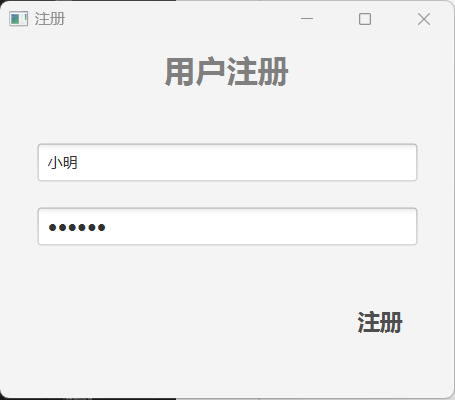
\includegraphics[width=0.5\textwidth]{pictures/12}
    \caption{完成注册}
\end{figure}
回到登录页面,进行登录
\begin{figure}[H]
    \centering
    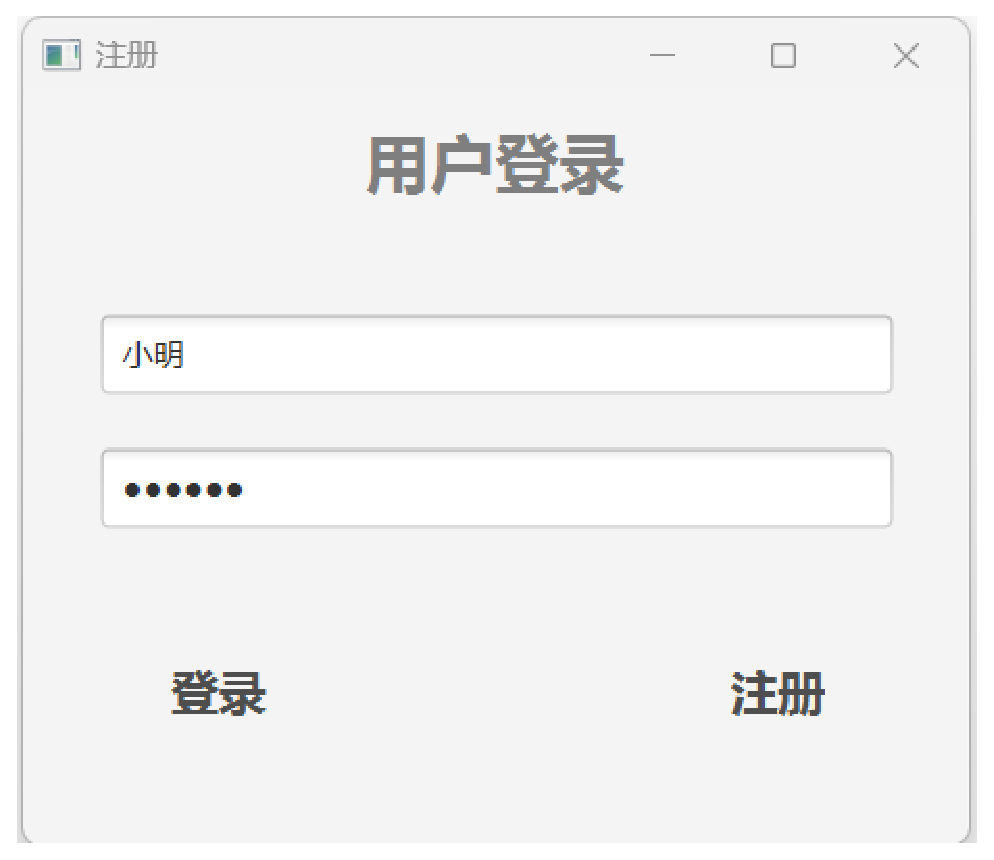
\includegraphics[width=0.5\textwidth]{pictures/13}
    \caption{完成登录}
\end{figure}
进入主界面
\begin{figure}[H]
    \centering
    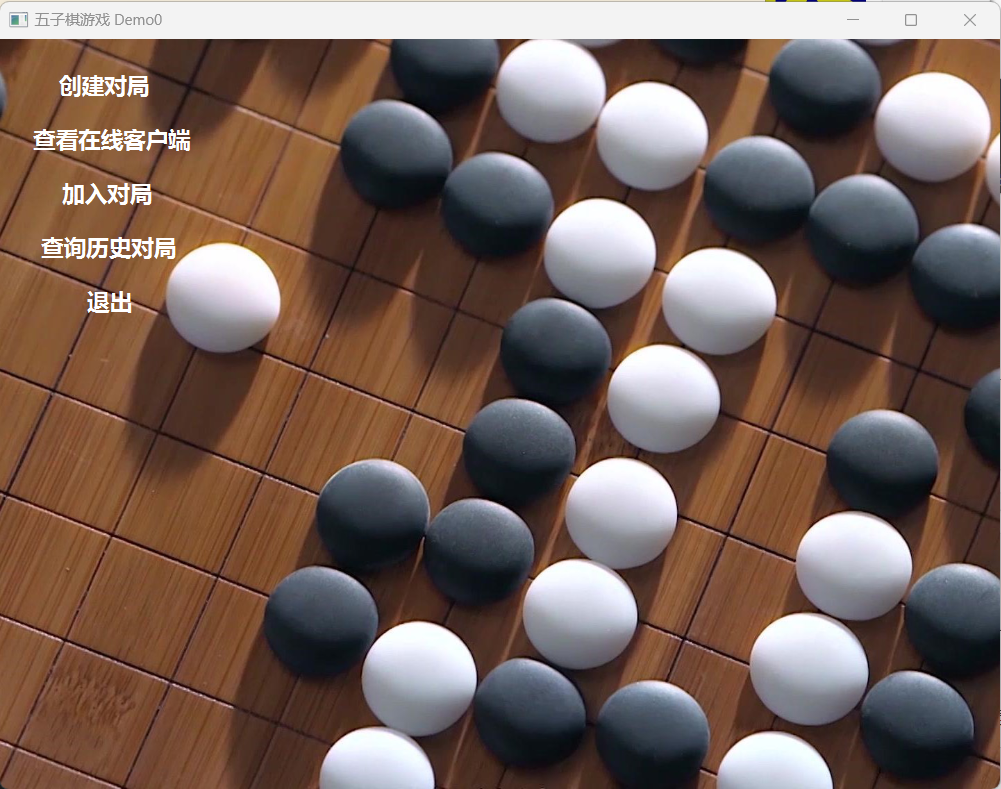
\includegraphics[width=0.5\textwidth]{pictures/14}
    \caption{主界面}
\end{figure}
查看在线客户端
\begin{figure}[H]
    \centering
    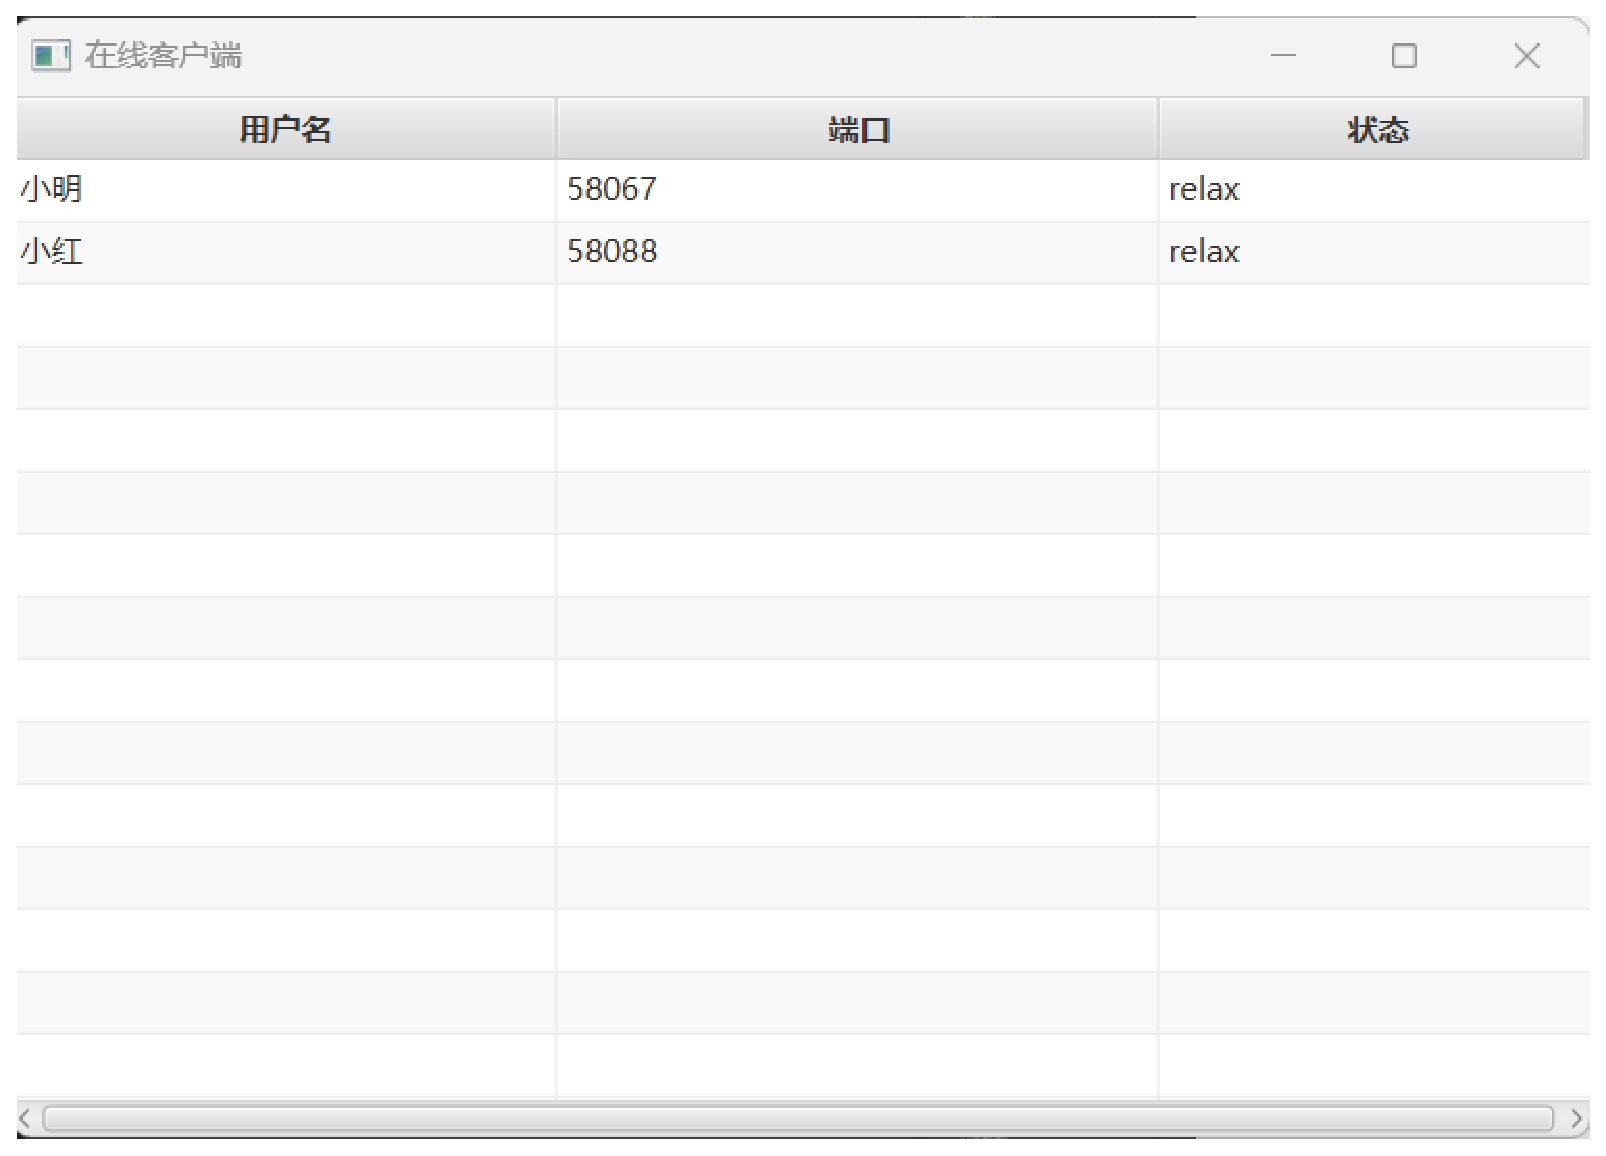
\includegraphics[width=0.5\textwidth]{pictures/17}
    \caption{在线客户端}
\end{figure}
点击创建对局
\begin{figure}[H]
    \centering
    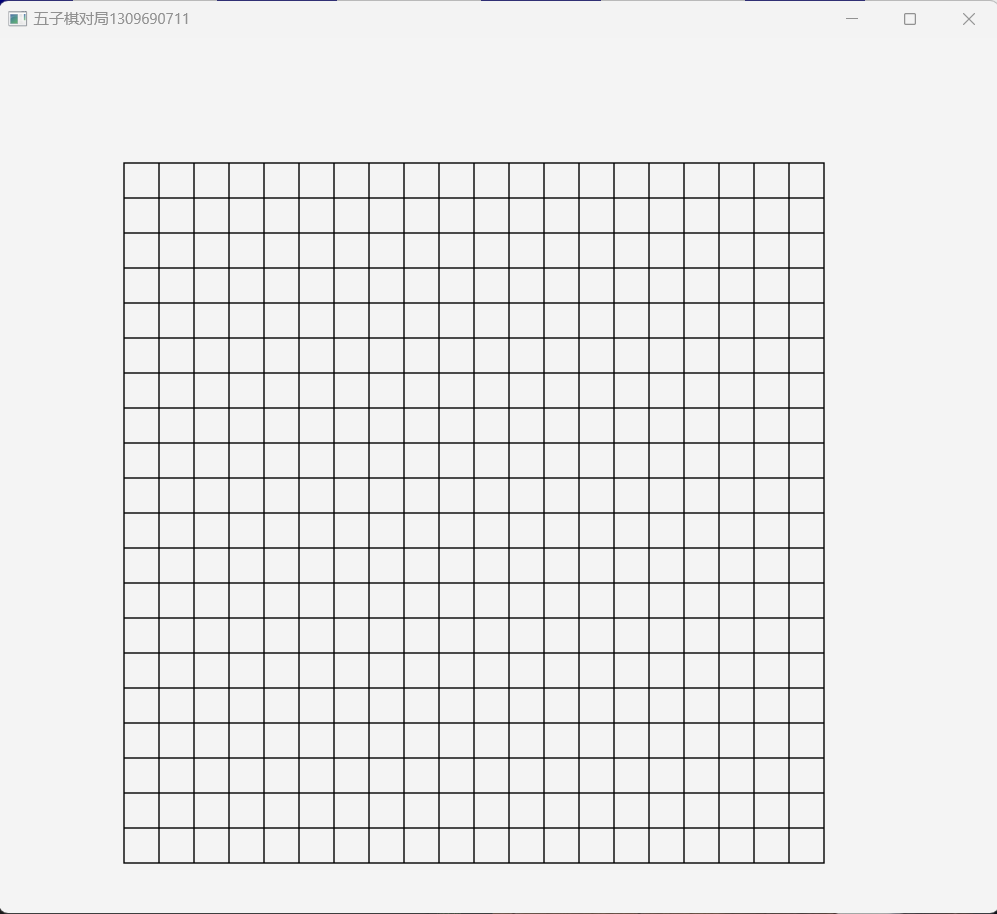
\includegraphics[width=0.8\textwidth]{pictures/18}
    \caption{创建对局}
\end{figure}
这时另一个客户端加入对局,对局开始
\begin{figure}[H]
    \centering
    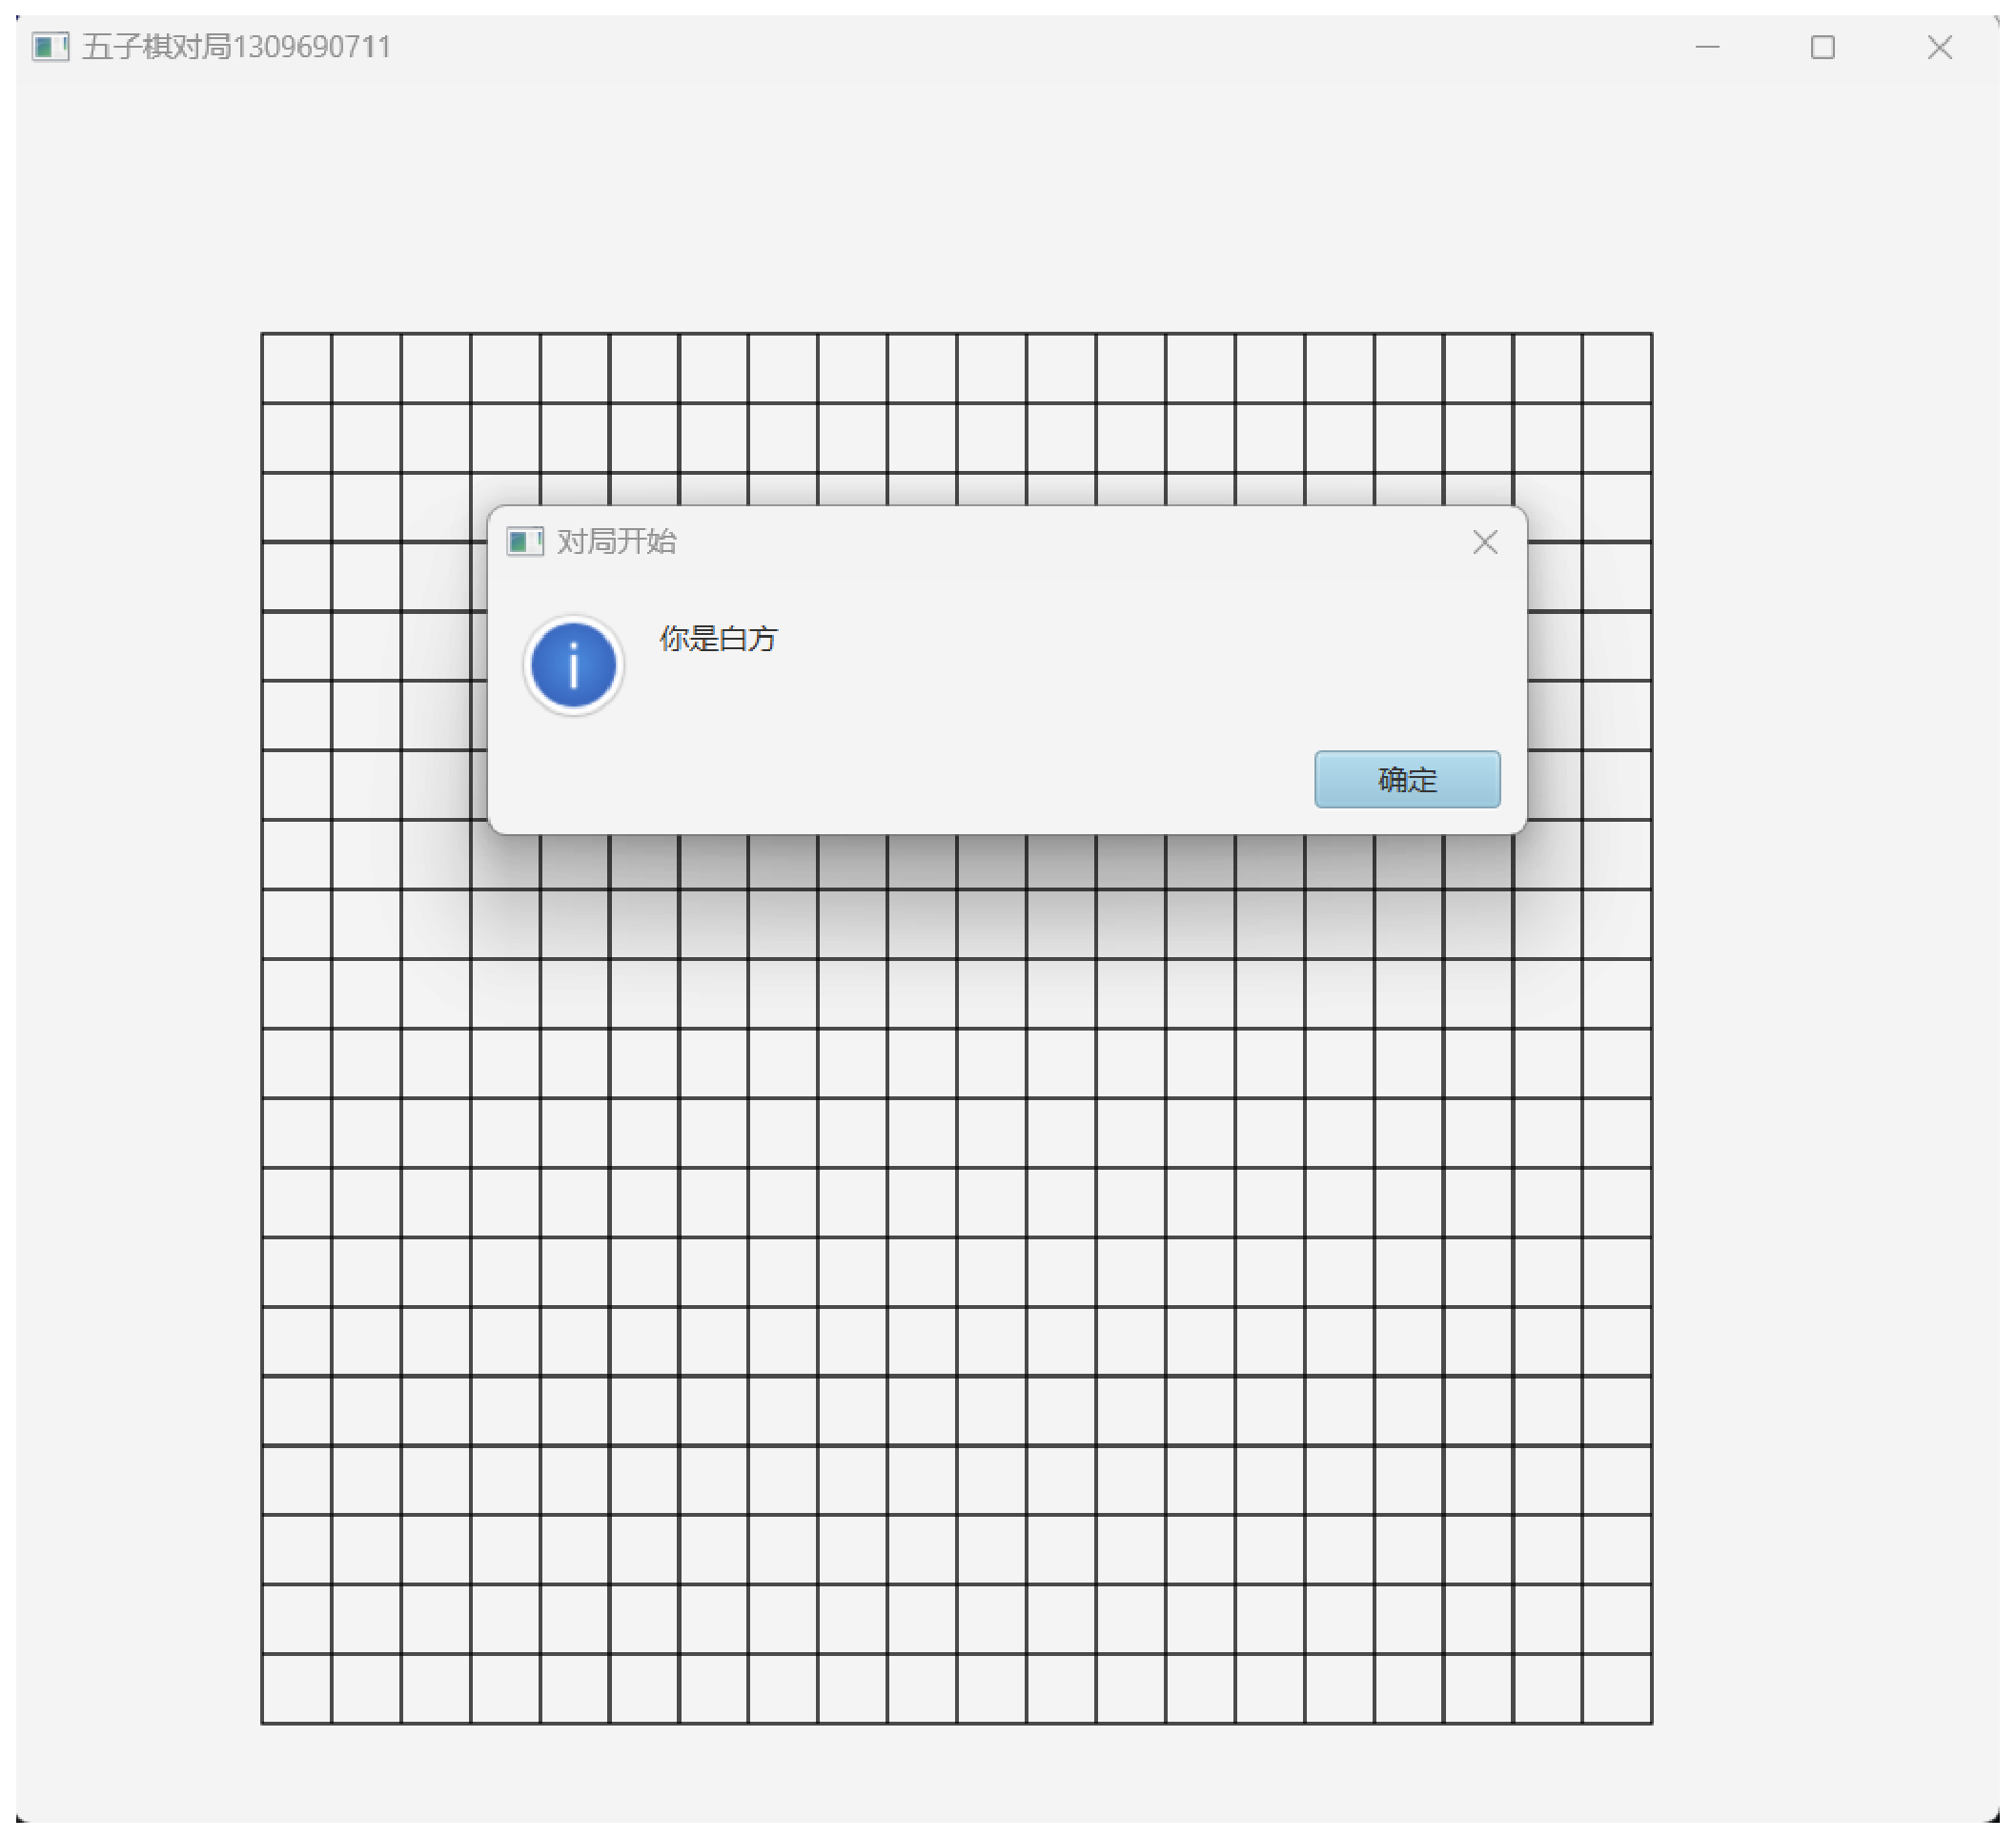
\includegraphics[width=0.8\textwidth]{pictures/19}
    \caption{对局开始}
\end{figure}
两边开始对局
\begin{figure}[H]
    \centering
    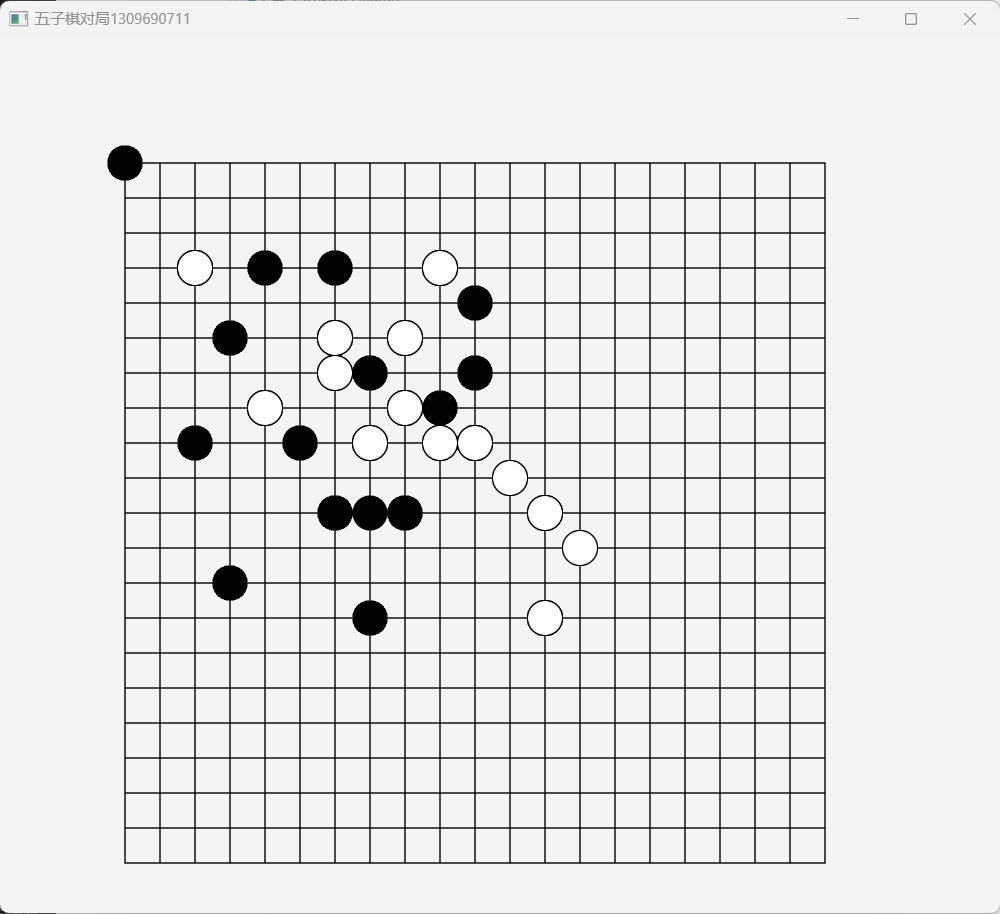
\includegraphics[width=0.8\textwidth]{pictures/20}
    \caption{对局中}
\end{figure}
白方赢得了对局
\begin{figure}[H]
    \centering
    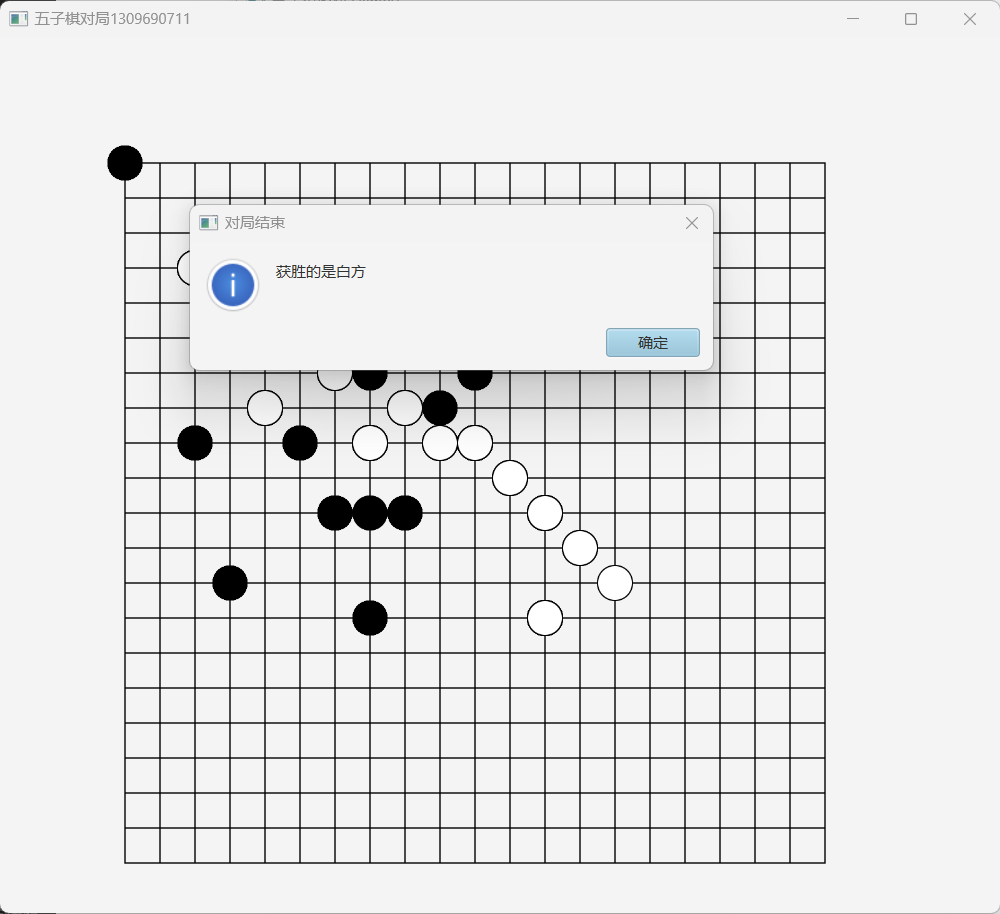
\includegraphics[width=0.8\textwidth]{pictures/21}
    \caption{对局结束}
\end{figure}
查看历史对局
\begin{figure}[H]
    \centering
    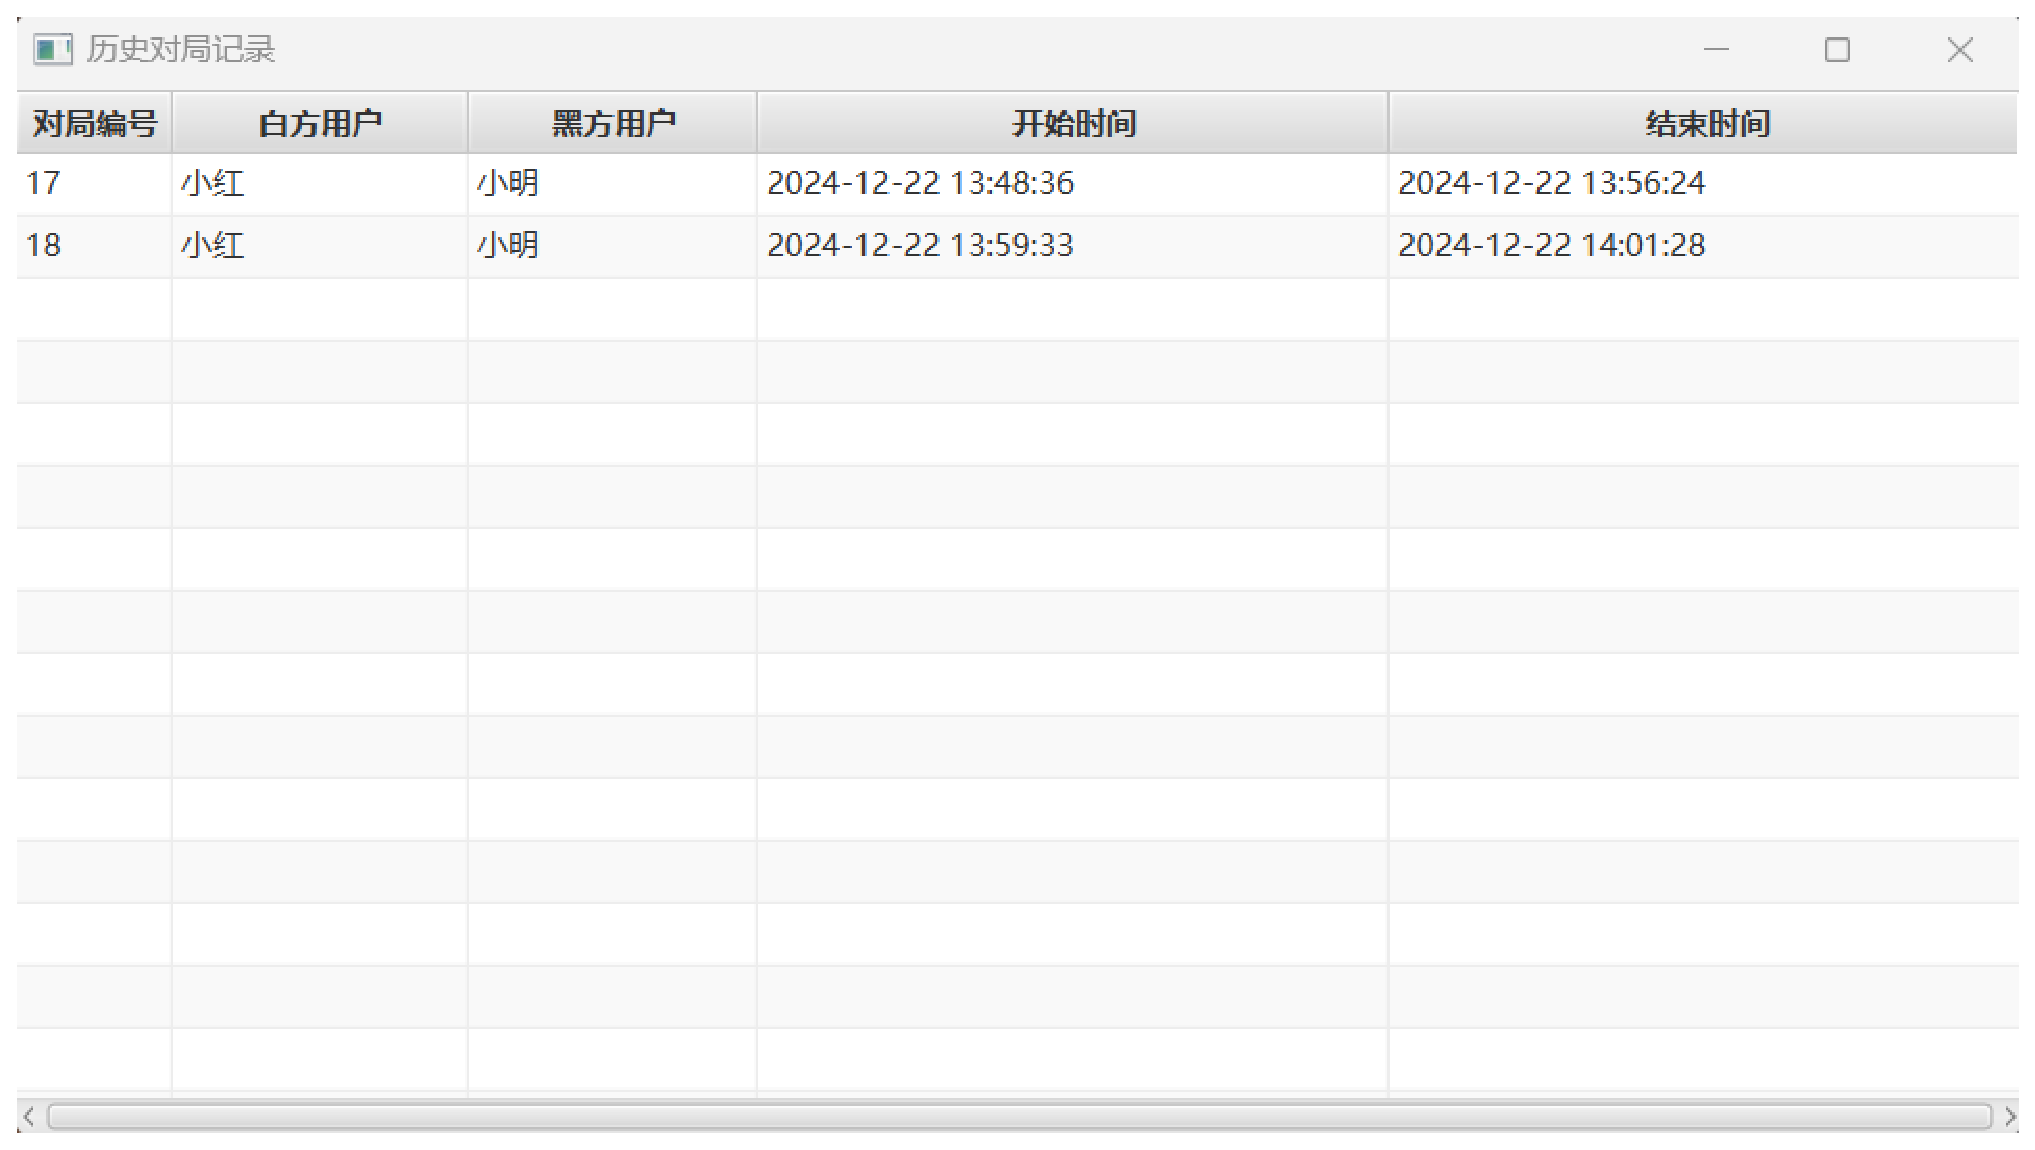
\includegraphics[width=0.8\textwidth]{pictures/22}
    \caption{历史对局}
\end{figure}
查看刚才对局的棋谱
\begin{figure}[H]
    \centering
    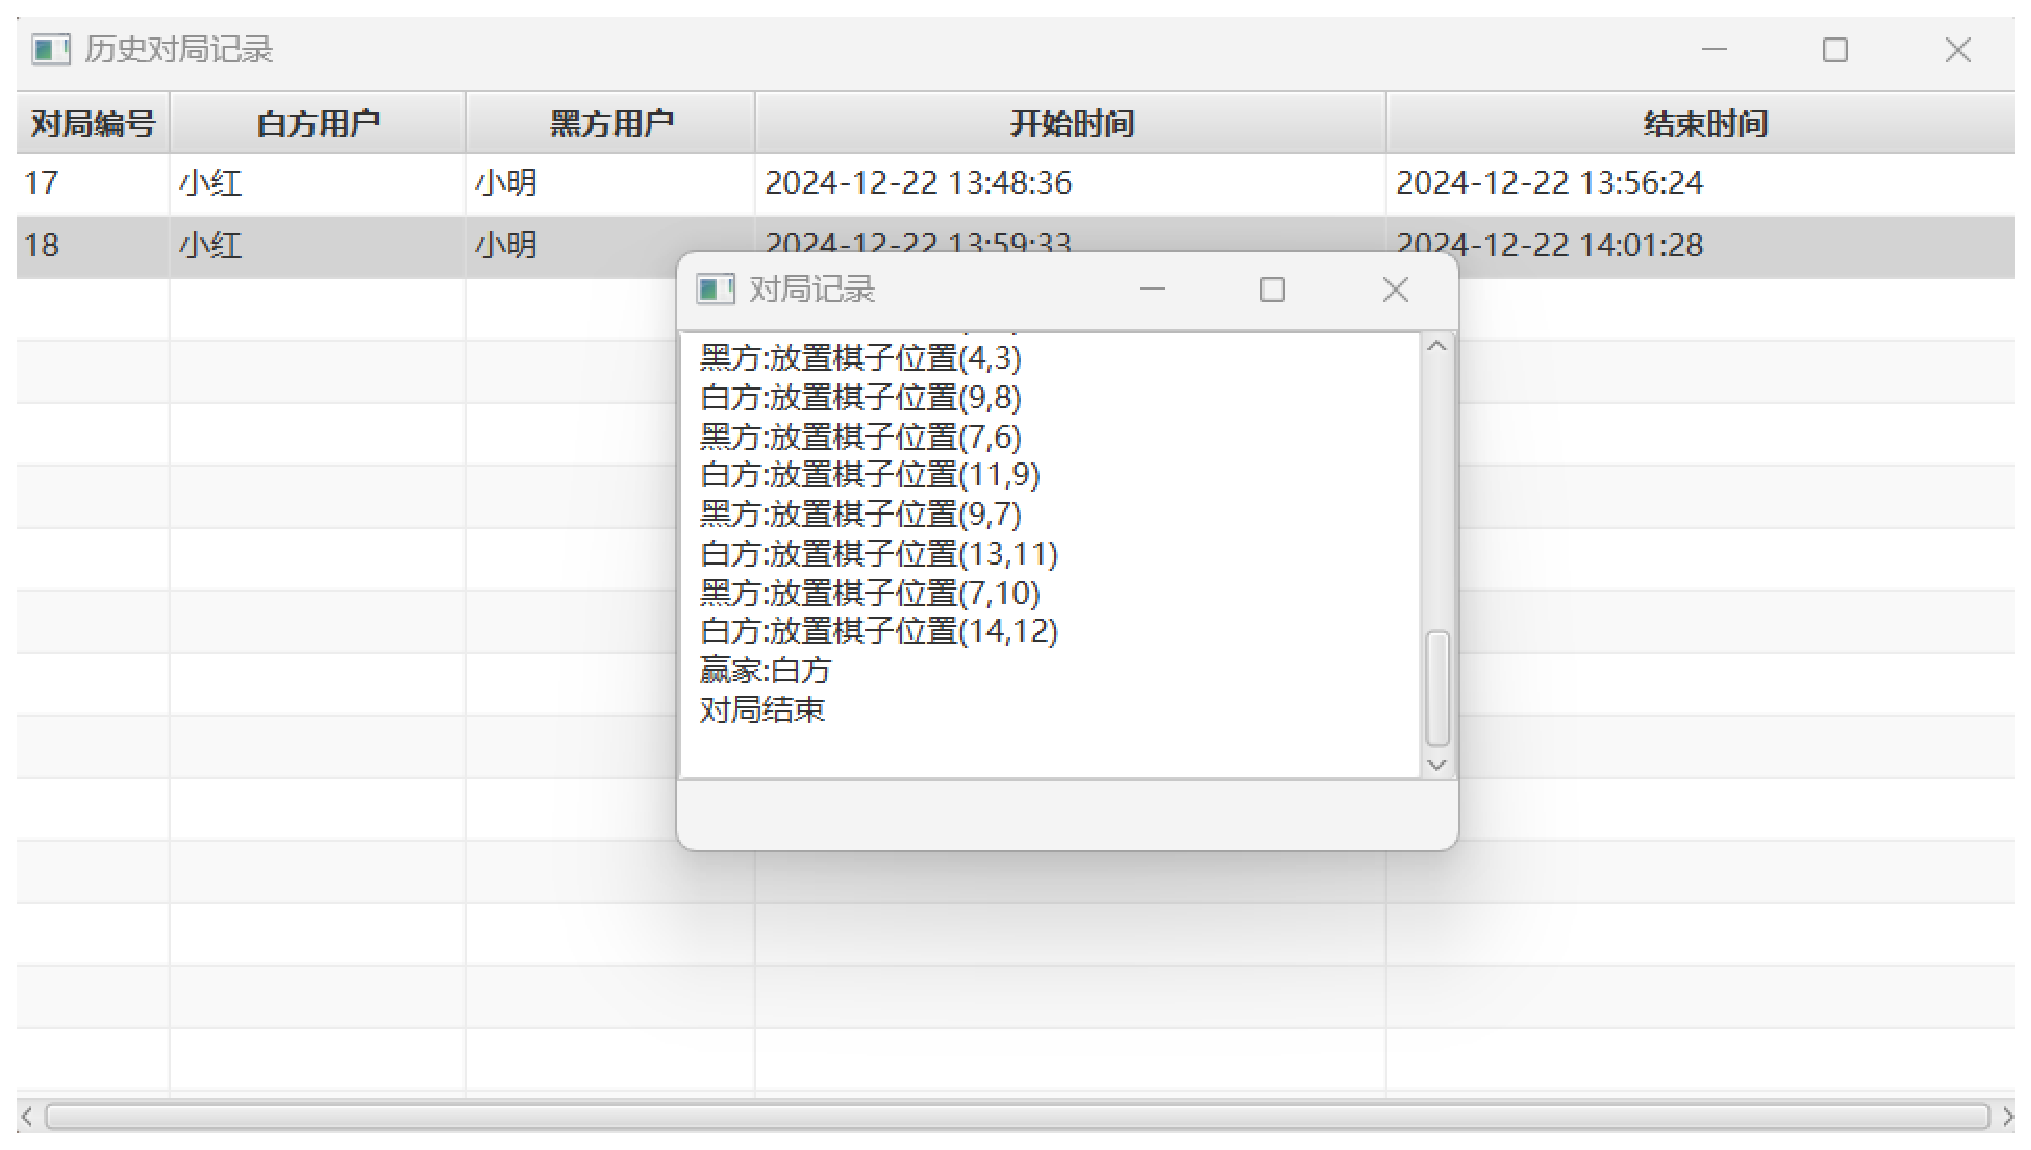
\includegraphics[width=0.8\textwidth]{pictures/23}
    \caption{对局棋谱}
\end{figure}
最后回到主界面退出客户端。

\section{总结}
在本次项目中,我使用Java语言,依靠网络编程、多线程编程、数据库操作和GUI设计方面的知识,初步搭建起了一个
五子棋在线对局的应用程序。

经过这次编程实践,我不仅巩固了在Java程序课上学习到的相关知识,也通过互联网学到了在课程之外的一些前沿知识。譬如,
在GUI的设计上,我通过JavaFx、FXML加上scene\ builder的设计模式,实现可视化、低代码地搭建GUI界面,简化了设计过程。
同时也引入了css的样式设计,使得我可以向写前端网页一样装饰我的GUI控件。

此外,和其他诸如网络聊天室之类的应用不同,本项目作为一个网络游戏程序,还需要保证输赢的可靠性和不可篡改性,保证用户的
恶意行为会被服务端所阻拦。因此,本项目在设计时也考虑到了可能存在的客户端恶意行为,将所有的对局判断、数据记录都放
在服务端上执行和储存,这样,即使有用户通过恶意篡改客户端,发送非法的操作时,服务端也能进行阻拦并保证对局的正确性。这
也是我在编写代码时花费时间最多的模块。

然而,由于本项目的编写时间有限,且本项目只是由个人完成的一次作业而已,还存在许多的复杂情况并没有被很好的考虑,还存在
很多有意思的功能没有被实现。譬如,本项目中用户加入对局时只能随机加入,并不能由自己选择。本项目的棋谱为文本形式,
没有使用可视化的棋盘来展现等。鉴于临近期末,有限的时间和精力都不太支持我继续深入开发项目,而只能遗憾止步于此。

但总而言之,通过本次项目实践,我加深了对Java面向程序设计的理解,代码管理和编程水平亦有提高,这就足够了。

\end{document}

